\chapter{Theoretical and Experimental Overview} \label{ch::theory_exp}
\ifpdf
\graphicspath{{Chapters/Theory/Figs/Raster/}{Chapters/Theory/Figs/PDF/}{Chapters/Theory/Figs/}}
\else \graphicspath{{Chapters/Theory/Figs/Vector/}{Chapters/Theory/Figs/}}
\fi

\section{Deep Inelastic Scattering}
To understand the structure of the nucleon it is useful to first introduce the
original process which described the nucleon as having a sub-structure.  This
process is the Deep Inelastic Scattering (DIS) process where a lepton impinges
on a nucleon denoted as

\begin{equation}
l(\ell) + N(P) \rightarrow l(\ell') + X(P_X),
\end{equation}
\noindent
where $l$ denotes a lepton, $N$ denotes a nucleon, $X$ represents all products
not detected and $\ell$, $\ell'$, $P$ and $P_X$ are the four momentum for their
respective lepton or nucleon.  This process is an electromagnetic reaction where
a lepton is scattered via virtual photon exchange with the nucleon.  The
leading order Feynman diagram for this reaction is shown in
Fig.~\ref{fig::DIS_LO}.

\begin{figure}[h!t]
  \centering
  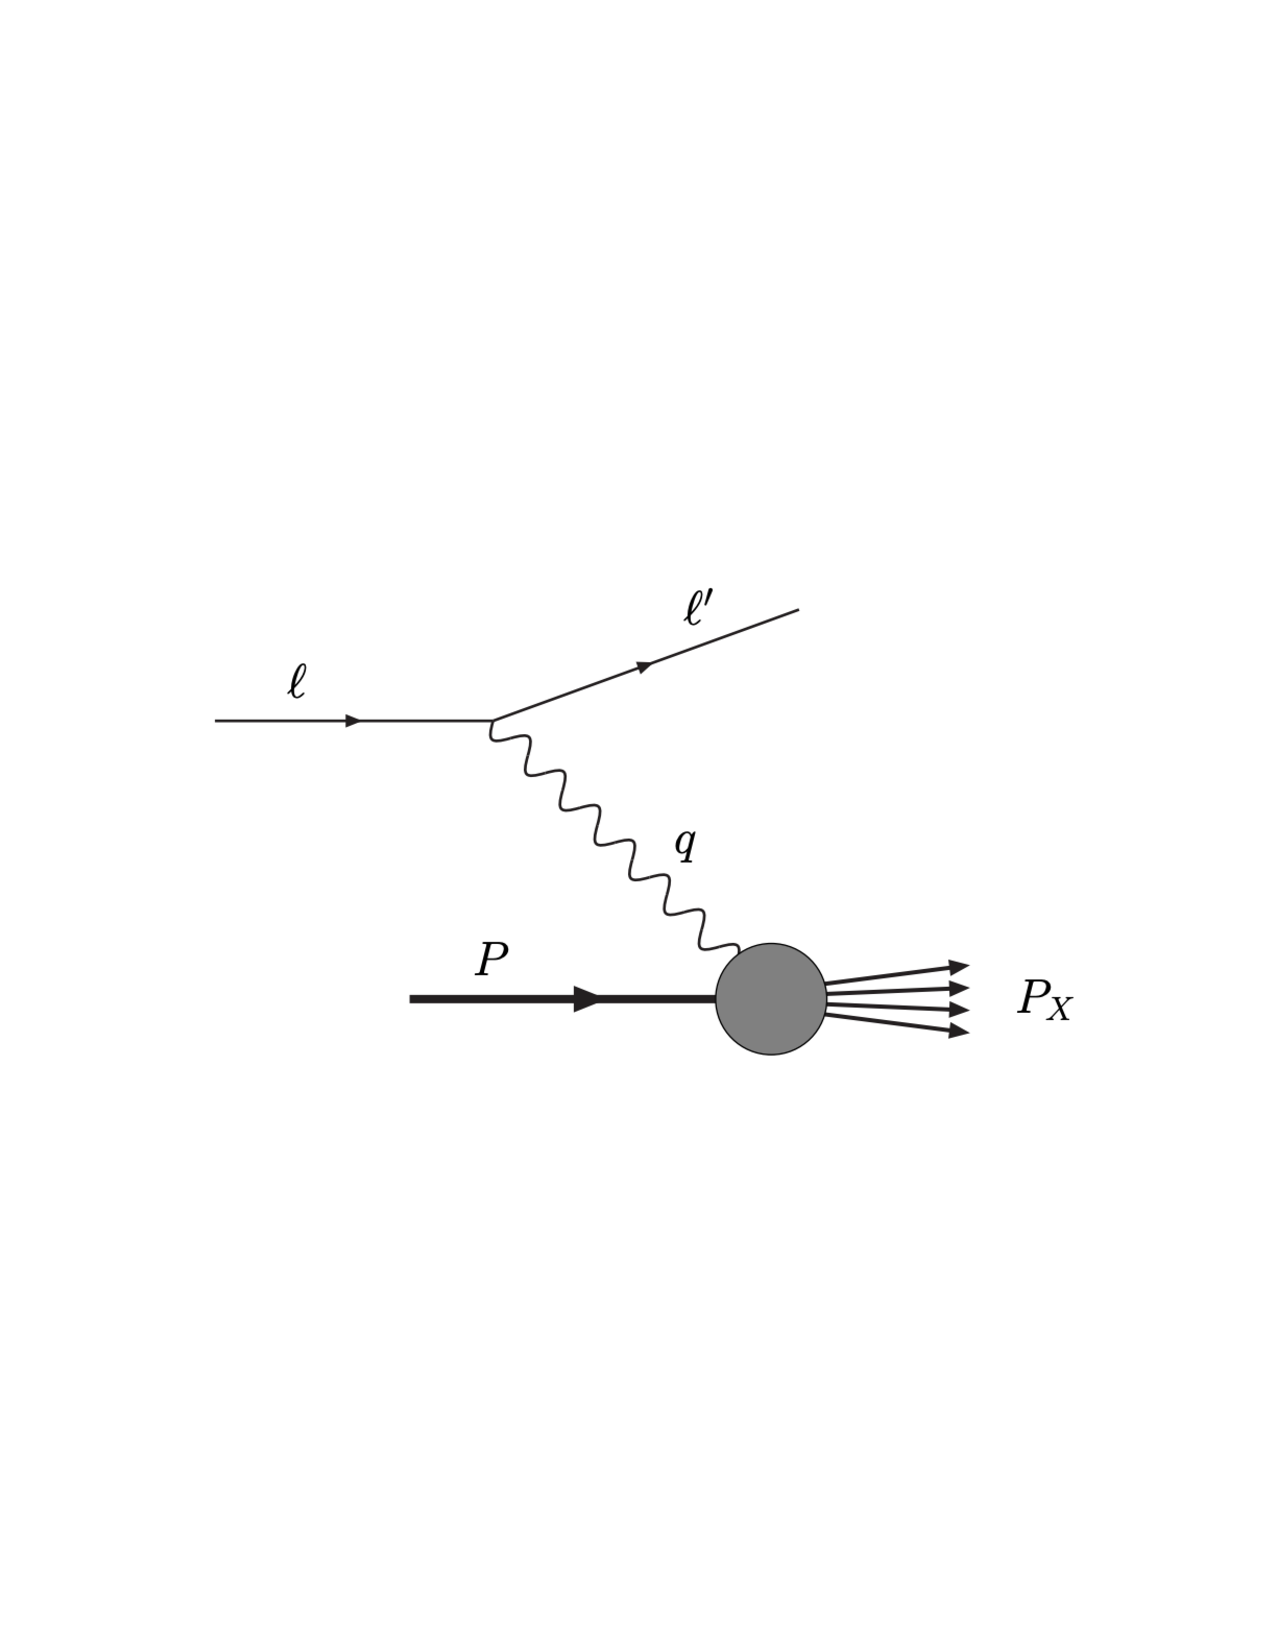
\includegraphics[width=0.5\textwidth, trim=3cm 9cm 3cm 9cm, clip]{DIS_LO}
  \caption{The leading order Feynman diagram for deep inelastic scattering}
  \label{fig::DIS_LO}
\end{figure}

DIS is traditionally studied with a high energy lepton beam and a fixed nuclear
target.  The initial state kinematics are described by

\begin{equation}
  s = (\ell+P)^2 \quad \mathrm{or} \quad E,
\end{equation}
\noindent
where $s$ is the center of mass energy and $E$ is the energy of the lepton beam.
The detected reaction kinematics in the lab frame are described by

\begin{multicols}{2}
  \noindent
  \begin{equation}
    \label{equ::DIS_Q2}
    Q^2 = -q^2 = -(\ell - \ell')^2 \approx EE'(1-\cos\theta )
  \end{equation}
  \begin{equation}
      \label{equ::BjorkenX}
      x = \frac{Q^2}{2P \cdot q} = \frac{Q^2}{2M\nu}
  \end{equation}
\end{multicols}

\begin{multicols}{2}
  \noindent
  \begin{equation}
    \nu = E - E'
  \end{equation} 
  \begin{equation}
    \label{equ::inelasticity}
    y = \frac{P \cdot q}{P \cdot \ell} = \frac{E - E'}{E} = \frac{\nu}{E}
  \end{equation} 
\end{multicols}

\begin{multicols}{2}
  \noindent
  \begin{equation}
    \label{equ::DIS_W}
    W^2 = (P+q)^2
  \end{equation}
\end{multicols}

\noindent
where $q$ is the virtual photon four momentum, $E'$ is the scattered lepton's
energy, $x$ is Bjorken x, $\nu$ is the change in energy of the scattered lepton,
$y$ is the inelasticity and $W^2$ is the invariant mass of the hadron final
state.  In the last relation from Eq.~\ref{equ::DIS_Q2}, $\theta$ is the
scattering angle of the lepton with respect to the beam and the approximation is
only true when the lepton mass is assumed to be zero.  This assumption and the
assumption that a quark's mass is zero will be made throughout this thesis.  In
Eq.~\ref{equ::BjorkenX}, $M$ is the nucleon mass.

In the parton model, section~\ref{sec::parton_model}, $x$ has the interpretation
as being the longitudinal momentum fraction of the struck parton with respect to
its parent hadron and therefore $x$ ranges between 0 and 1.  The inelasticity,
$y$, measures the proportional energy reduction of the lepton and therefore it's
value ranges between 0 and 1.

The process is called deep if $Q^2 >> M^2$ and inelastic if $y < 1$.  For
practical purposes, in experiments, the deep inelastic criteria corresponds to a
$Q^2 > 1~GeV$ and $W^2 > M^2$.  As can be seen in
Eq.~[\ref{equ::DIS_Q2}-\ref{equ::DIS_W}], not all the variables are independent.
DIS is described by two independent variables usually given by ($x$, $Q^2$) or
($x$, $y$).  For reference, in the limit as $y \to \; 1$ the process becomes
elastic scattering and can then be described by only one independent variable.

The differential cross-section for DIS is defined as~\cite{Barone:2001sp}
\begin{equation}
  \label{equ::DIS_xsection}
  \mathrm{d}\sigma =
  \frac{1}{4P\cdot \ell}\frac{e^4}{Q^4} L_{\mu\nu}W^{\mu\nu}
  2\pi\frac{\mathrm{d}^3\ell'}{(2\pi)^32E'}
\end{equation}
\noindent
where $L_{\mu\nu}$ is the leptonic tensor and $W^{\mu\nu}$ is the hadronic
tensor.  The leptonic tensor describes free leptons and can therefore be
calculated in perturbation theory.  It can be decomposed into a systematic
spin-independent tensor and an anti-symmetric spin-dependent tensor.  Summing
over all the possible spins of the lepton beam, the leptonic tensor is

\begin{equation}
  L_{\mu\nu} = 2\Big(\ell_{\mu}\ell'_{\nu} + \ell_{\nu}\ell'_{\mu} -
  g_{\mu\nu}\ell \cdot \ell' \Big) +
  2m\epsilon_{\mu\nu\rho\sigma}s^{\rho}q^{\sigma}
\end{equation}
\noindent
where $m$ is the lepton mass and $s^{\rho}$ is the spin four vector of the
lepton.

Generically the hadronic tensor is defined as
\begin{equation}
  W^{\mu\nu} = \frac{1}{2\pi}
  \int \mathrm{d}^4\xi e^{iq \cdot \xi}
  \langle PS | J^{\mu}(\xi)J^{\nu}(0) | PS \rangle
\end{equation}
\noindent
where $J$ is an electromagnetic current and $|PS \rangle$ represents the nucleon
with momentum $P$ and spin $S$.  The hadronic tensor describes a hadron bound
together by quantum chromo-dynamics (QCD).  As of yet there is no known
technique for calculating the hadronic tensor in a perturbation theory or
otherwise.  Instead the hadronic tensor can be written in the most general
Lorentz invariant form using structure functions to parameterize the
non-perturbative nature of the tensor.  With the use of these structure
functions, the differential DIS cross-section can be written
\begin{equation}
  \label{equ::DIS_diffxsection}
  \frac{\mathrm{d}\sigma}{\mathrm{d}x\mathrm{d}y} =
  \frac{8\pi\alpha^2ME}{Q^4}
  \Big\{
  xy^2F_1(x, Q^2) + \Big(1-y\Big)\frac{F_2(x, Q^2)}{x}
  + c_1(y, \frac{Q^2}{\nu}) g_1(x, Q^2) + c_2(y, \frac{Q^2}{\nu}) g_2(x, Q^2)
  \Big \}
\end{equation}
\noindent
where $\alpha$ is the electromagnetic coupling constant; $F_1$, $F_2$, $g_1$,
$g_2$ are structure functions; and $c_1$ and $c_2$ are functions which depend on
the polarization of the target.  The SLAC collaboration measured the structure
functions, $F_1$ and $F_2$, and found mild variations as a function of
$Q^2$~\cite{Bloom:1969kc,Breidenbach:1969kd}.  This phenomenon now known as
Bjorken scaling lead to the theory of the parton model where the DIS reaction no
longer depends on $Q^2$~\cite{Bjorken:1969ja}.  Fig.~\ref{fig::F2} shows the
$F_2$ structure function which is approximately constant as a function of $Q^2$.

\begin{figure}[h!t]
  \centering
  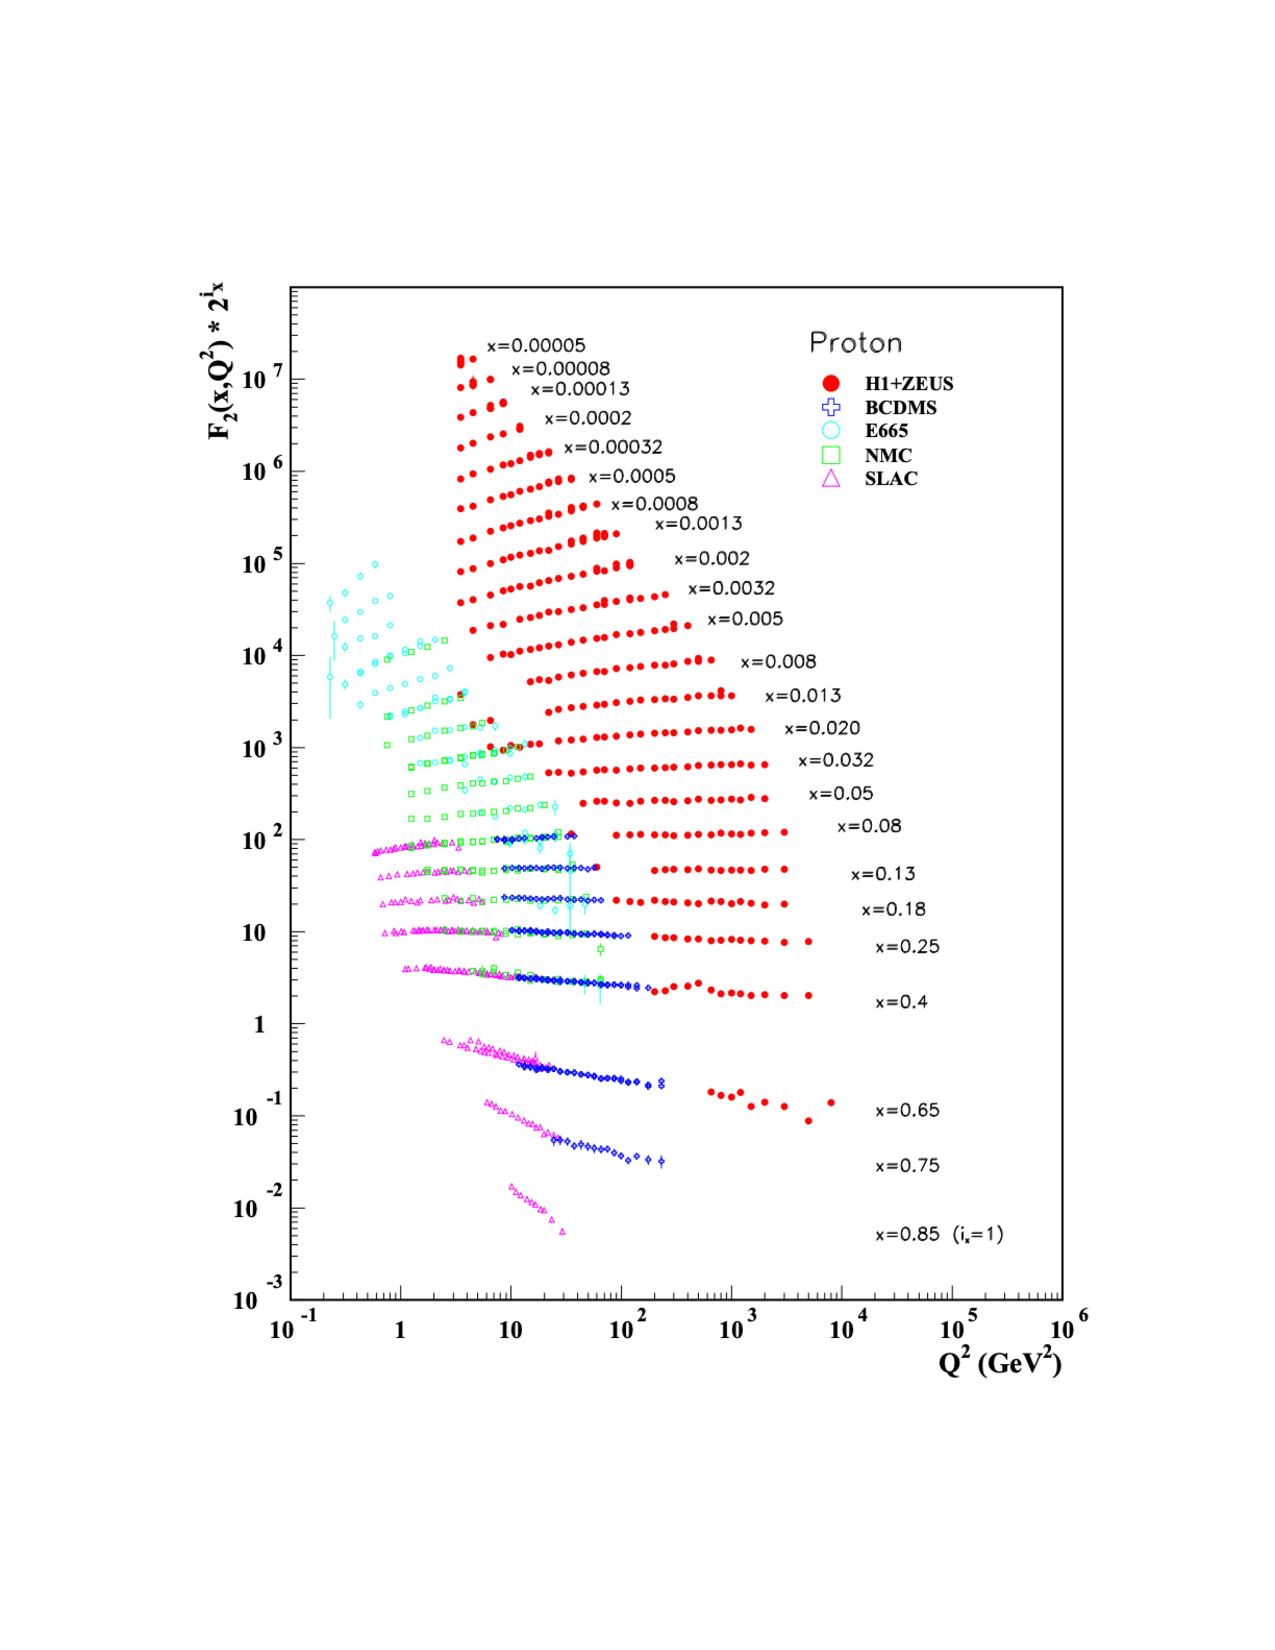
\includegraphics[width=0.5\textwidth, trim=3cm 4cm 3cm 4cm, clip]{F2}
  \caption{The $F_2$ structure function measured by several experiments.  Note
    that the data is shifted up by a factor $2^{i_x}$ to see the $x$ dependence.
    Image taken from~\cite{Tanabashi:2018oca}}
  \label{fig::F2}
\end{figure}


\section{The Parton Model} \label{sec::parton_model}
The parton model is described in an infinite momentum frame which for practical
measurements is defined as the frame where the nucleon is moving with momentum
larger than it's invariant mass.  In the parton model the nucleon, in high
energy scattering processes, is considered to be composed of point like
constituent mass-less particles called partons.  At high energy scattering the
QCD strong force, binding the partons together, becomes asymptotic small and
therefore the partons appear to be free.  The cross-section in DIS can then be
described as a lepton scattering incoherently off a free parton in the nucleon.
In the parton model the hadron tensor for scattering off a quark can be written
as~\cite{Barone:2001sp}

\begin{dmath}
  W^{\mu\nu} = \frac{1}{2\pi} \sum_q e_q^2 \sum_X
  \int \frac{\mathrm{d}^3 P_X}{(2\pi)^32E_X}
  \int \frac{\mathrm{d}^4k}{(2\pi)^4}
  \int \frac{\mathrm{d}^4k'}{(2\pi)^4} \delta(k^{\prime2}) 
       \times [\bar{u}(k')\gamma^{\mu}\langle X | u(k) | PS \rangle] 
       \times [\bar{u}(k')\gamma^{\nu}\langle X | u(k) | PS \rangle]
       \times (2\pi)^4\delta^{(4)}(P-k-P_X)(2\pi)^4\delta^{(4)}(k+q-k'),
\end{dmath}
\noindent
where $e_q$ is the electric charge of quark flavor $q$ and $u(\bar{u})$
is a free Dirac spinor.  This hadronic tensor can be simplified by introducing
the quark-quark correlation matrix as

\begin{equation}
  \Theta_{ij}(k, P, S) =
  \sum_X \int \frac{\mathrm{d}^3 P_X}{(2\pi)^32E_X}(2\pi)^4\delta^{(4)}(P-k-P_X)
  \times \langle PS | \phi_j(0) | X \rangle \langle X | \phi_i(0) | PS \rangle,
\end{equation}
\noindent
where $\phi(\xi) = e^{-ip \cdot \xi}u(p)$ is a quark field.  Using the
quark-quark correlation matrix, the hadronic tensor can be written as

\begin{equation}
  W^{\mu\nu} = \sum_q e_q^2 \int \frac{\mathrm{d}^4k}{(2\pi)^4}
  \int \frac{\mathrm{d}^4k'}{(2\pi)^4} \delta(k^{\prime2})
  (2\pi)^4\delta^{(4)}(k+q-k')\times \mathrm{Tr}
  [ \Theta \gamma^{\mu}\slashed{k'}\gamma^{\nu} ].
\end{equation}
\noindent
In the cases of unpolarized or longitudinally polarized DIS the lead order
contributing terms from the quark-quark correlator
are~\cite{Mulders:1995dh,Boer:1997nt,Bacchetta:2006tn}

\begin{equation}
  \label{equ::simpleQQcorr}
  \Theta = \frac{1}{2}
  \Big(
  f_1(x)\slashed{P} +
  g_{1L}(x)\lambda\gamma_5\slashed{P}
  \Big)
\end{equation}
\noindent
where $\lambda$ is the longitudinal polarization of the hadron.  In this case,
the hadronic tensor simplifies to a symmetric contribution and an anti-symmetric
contribution as~\cite{Barone:2001sp}

\begin{equation}
  \label{equ::simpleHadronTensor}
  W^{\mathrm{symmetric}}_{\mu\nu} = \frac{1}{P\cdot q} \sum_q e_q^2
  \Big( (k_{\mu}+q_{\mu})P_{\nu} + (k_{\nu}+q_{\nu})P_{\mu}-g_{\mu\nu}
  \Big) f_1^q(x),
\end{equation}
\begin{equation}
  W^{\mathrm{anti-symmetric}}_{\mu\nu} =
  \lambda\epsilon_{\mu\nu\rho\sigma}(k_{\nu}+q_{\nu})P^{\rho}\sum_q e^2_q
  g^q_{1L}(x),
  \label{equ::Wantisymmetric}
\end{equation}
\noindent
where in Eq.~\ref{equ::simpleQQcorr}-\ref{equ::Wantisymmetric}, $f_1$ and $g_1$
are parton distribution functions (PDFs).

$f_1$ is interpreted as the quark number density and $g_{1L}$ is interpreted as
the total quark helicity distribution in a hadron.  $f_1$ refers to the density
of unpolarized quarks in a hadron and $g_{1L}$ refers to the net density of
quarks longitudinally polarized in the same longitudinal direction as the
hadron.  To make this explicit, $f_1$ and $g_{1L}$ can be written

\begin{multicols}{2}
  \noindent
  \begin{equation}
    f_1 = f_1^{+} + f_1^{-},
  \end{equation}
  \begin{equation}
    g_{1L} = f_1^{+} - f_1^{-},
  \end{equation}
\end{multicols}
\noindent
where +(-) denotes the helicity.  To be clear while there is a relationship
between the two functions, Eq.~\ref{equ::g1_g1l_relation}, the parton
distribution $g_{1L}$ is not the same as the structure function $g_1$.

The unpolarized quark number density, $f_1$, has been extracted from global
analysis of several experiments~\cite{Rojo_2015}.  Fig.~\ref{fig::NNPDF_10GeV}
shows the current $xf_1$ values and confidence intervals for different quarks
and gluons in the proton.

\begin{figure}[h!t]
  \centering 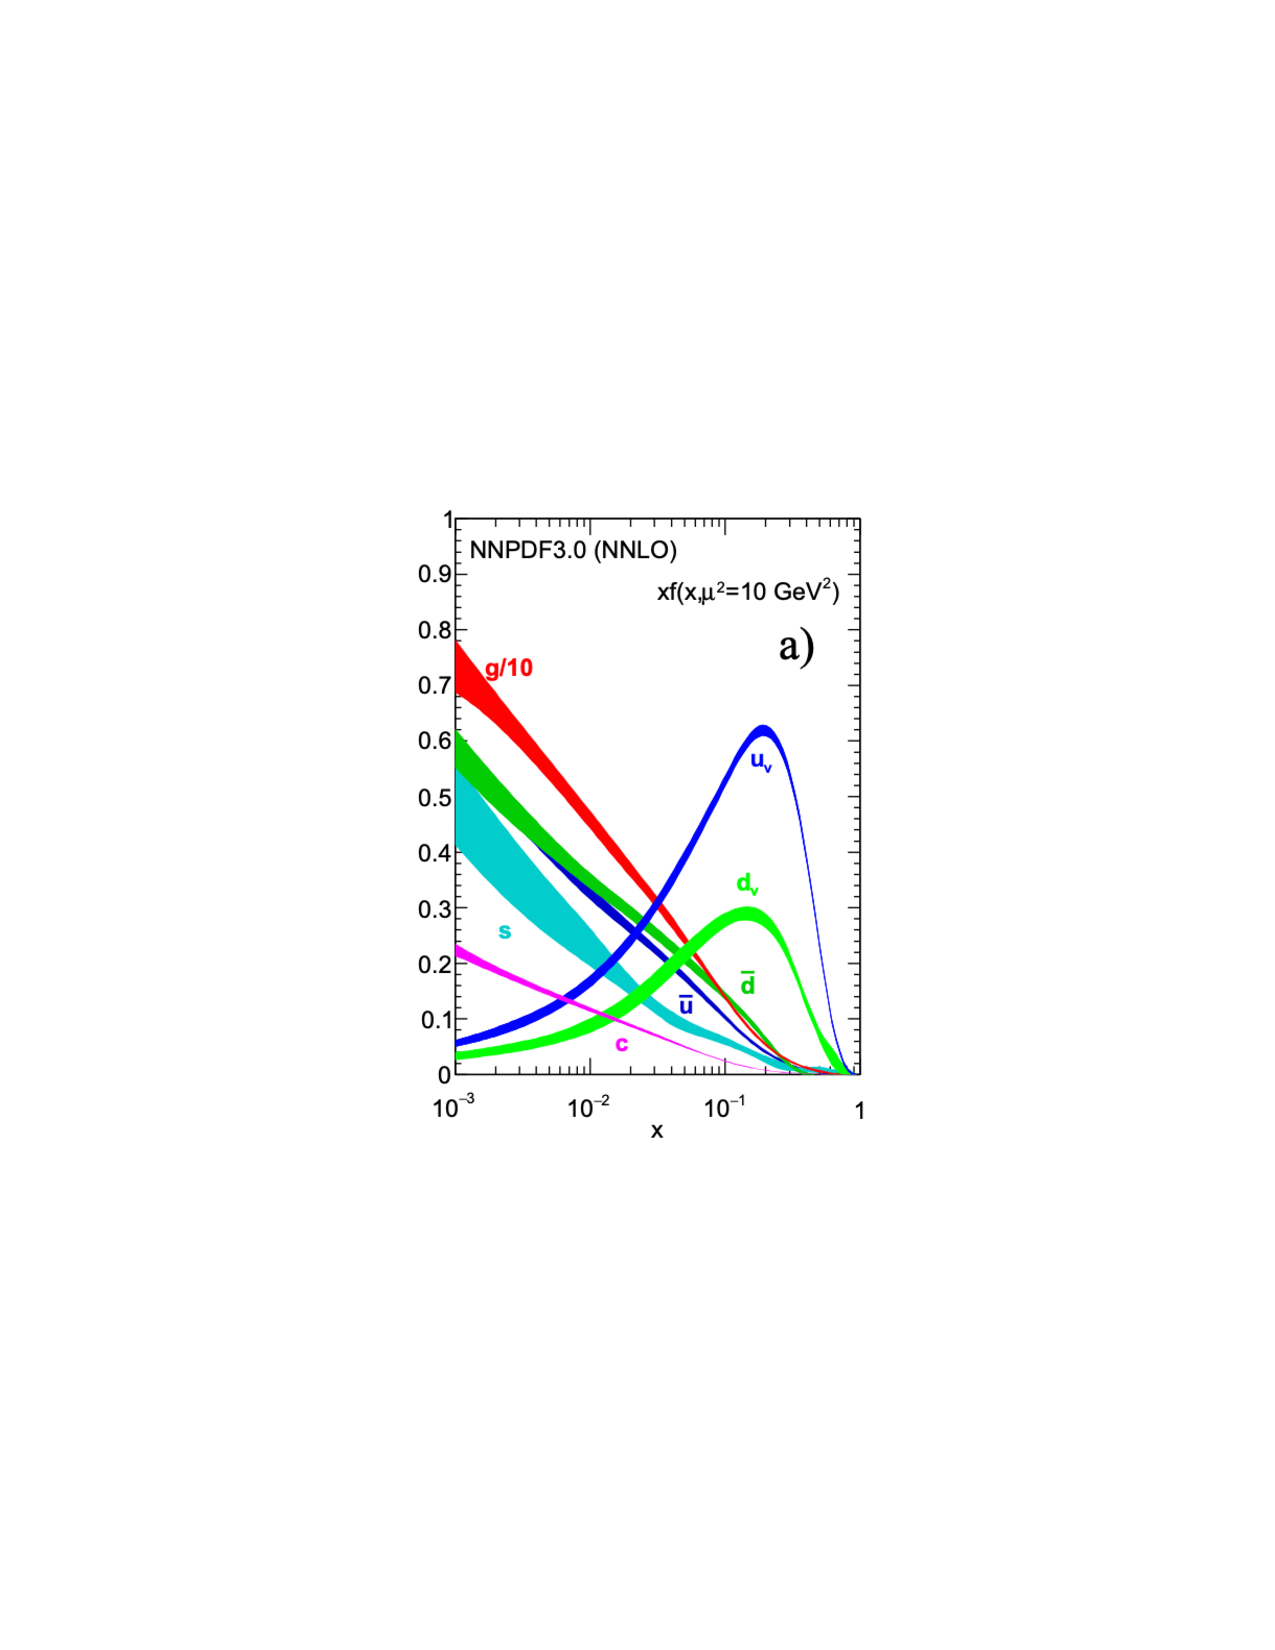
\includegraphics[width=0.5\textwidth,trim=6cm 9cm 6cm 8cm,
    clip]{NNPDF_10GeV}
  \caption{The unpolarized parton distribution functions times the momentum
    fraction.  The different colors correspond to different quarks or gluons.
    Image taken from~\cite{Tanabashi:2018oca}}
  \label{fig::NNPDF_10GeV}
\end{figure}

The longitudinal spin structure, $g_{1L}$, has also been measured at SMC,
HERMES, and COMPASS~\cite{Adeva:1997is,PhysRevLett.92.012005,Savin:2011zz}.  The
global analysis fit is shown in Fig.~\ref{fig::Proton_g1L} using the
parameterizations from NNPDF2014, AAC2008, DSSV2008 and
LSS2010~\cite{Harland-Lang:2016yfn,Abt:2016vjh,Nocera:2014gqa,Hirai:2008aj}.

\begin{figure}[h!t]
  \centering 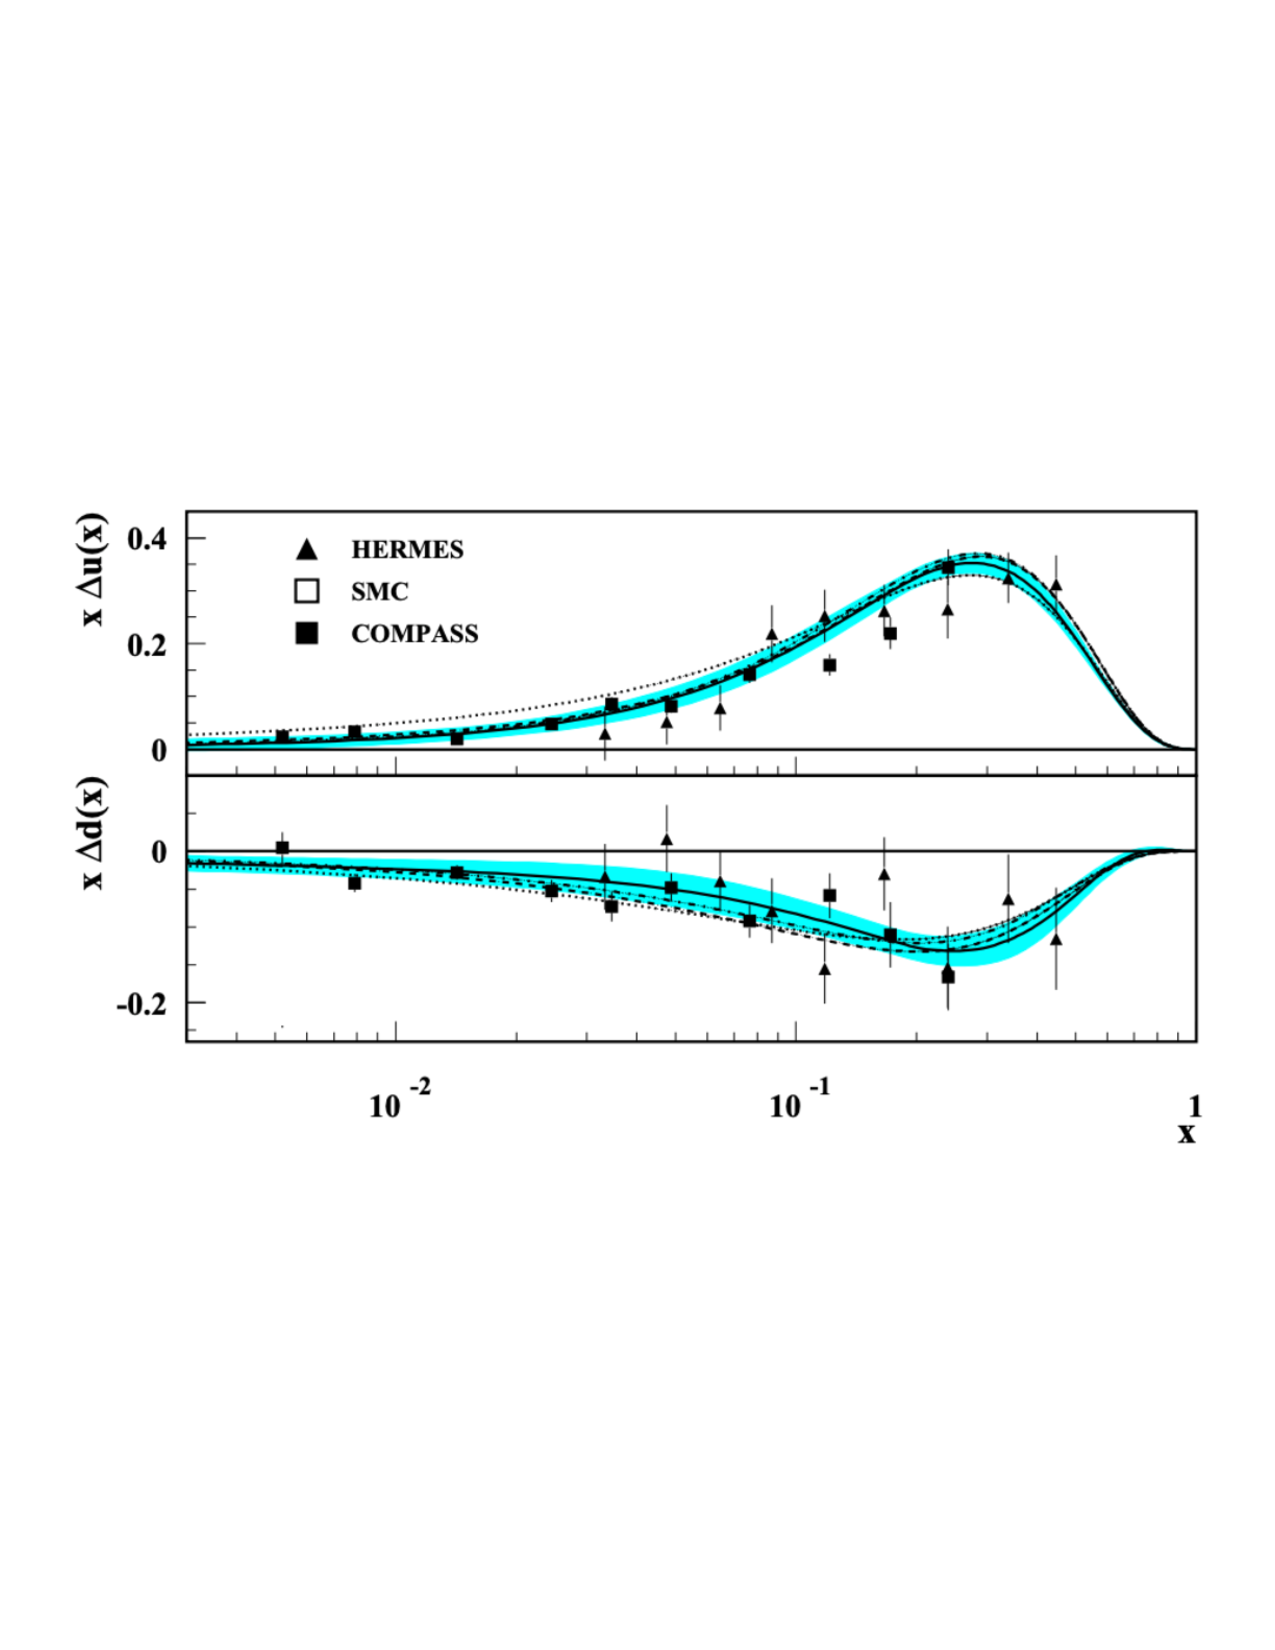
\includegraphics[width=0.5\textwidth,trim=1cm 8cm 1cm 8cm,
    clip]{Proton_g1L}
  \caption{The longitudinally polarized parton distribution functions times the
    momentum fraction for the u-quark (top) and the d-quark (bottom) in a
    proton.  Image taken from~\cite{Tanabashi:2018oca}}
  \label{fig::Proton_g1L}
\end{figure}

In the parton model the structure function $F_1$ and $F_2$ are related to each
other and to the unpolarized quark number as
\begin{equation}
  F_2(x) = 2xF_1(x) = \sum_q e_q^2x\Big(f^q_1 + f^{\bar{q}}_1 \Big)
\end{equation}
which is known as the Callan-Gross relation~\cite{PhysRevLett.22.156}.  As well
the structure function $g_1$ is related to the helicity distribution, $g_{1L}$,
as
\begin{equation}
  g_1(x) = \frac{1}{2} \sum_q e^2_q g_{1L}(x).
  \label{equ::g1_g1l_relation}
\end{equation}


\section{Transverse Momentum Dependence}
In deep inelastic scattering the detected final state lepton is not sensitive to
the parton's transverse momentum.  That is when measuring the DIS
cross-section, all transverse parton momentums are possible which therefore
means the scattered parton's transverse momentum is integrated over.  As a
result, DIS cannot be used to study parton's transverse momentum dependence.
The Drell-Yan process~\ref{sec::DY} and the SIDIS process~\ref{sec::SIDIS}
however are sensitive to the internal transverse momentum of the partons.  In
the limit of small transverse momentum compared to the virtual photon momentum,
the most generic leading order quark-quark correlator including the transverse
parton momentum can be
written~\cite{Mulders:1995dh,Boer:1997nt,Bacchetta:2006tn}

\begin{dmath}
  \label{equ::GeneralQQcorrelator}
  \Theta = \frac{1}{2}\Big[ f_1(x,k_{\bot})\slashed{P} +
    \frac{1}{M}h_1^{\bot}(x,k_{\bot})\sigma^{\mu\nu}k_{\mu}P_{\nu} +
    g_{1L}(x,k_{\bot})\lambda\gamma_5\slashed{P} +
    \frac{1}{M}g_{1T}(x,k_{\bot})\gamma_5\slashed{P}(k_{\bot} \cdot S_{\bot}) +
    \frac{1}{M}h_{1L}(x,k_{\bot})\lambda
    i\sigma_{\mu\nu}\gamma_5P^{\mu}k_{\bot}^{\nu} +
    h_1(x,k_{\bot})i\sigma_{\mu\nu}\gamma_5P^{\mu}S_{\bot}^{\nu} +
    \frac{1}{M^2}h_{1T}^{\bot}(x,k_{\bot})i\sigma_{\mu\nu}\gamma_5P^{\mu} \Big(
    k_{\bot} \cdot S_{\bot}k_{\bot}^{\nu} - \frac{1}{2}k_{\bot}^2S_{\bot}^{\nu}
    \Big ) +
    \frac{1}{M}f_{1T}^{\bot}(x,k_{\bot})\epsilon^{\mu\nu\rho\sigma}\gamma_{\mu}P_{\nu}k_{\rho}S_{\sigma}
    \Big],
\end{dmath}
\noindent
where $k_{\bot}$ denotes the transverse parton momentum and $S_{\bot}$ denotes
the transverse hadron spin.  Eq.~\ref{equ::GeneralQQcorrelator} includes eight
transverse momentum dependent (TMD) PDFs which are functions of $x$ and
$k_{\bot}$.

The notation used to depict the TMD functions is the so-called Amsterdam
notation.  The letters represent the different quark polarizations where
$f,\;g,\;h$ stand for unpolarized, longitudinally polarized and transversely
polarized respectively.  The subscript 1 denotes leading order and the
subscripts $T$ and $L$ denote a transversely polarized hadron and a
longitudinally polarized hadron respectively.  Finally the superscript $\bot$
denotes that the distribution is the coefficient of a term where the in which
the parton's transverse momentum Lorentz indices are not contracted.
Fig.~\ref{fig::TMDs} organizes the TMDs by nucleon and quark polarizations and
gives a visual of each TMD's interpretation.

\begin{figure}[h!t]
  \centering
  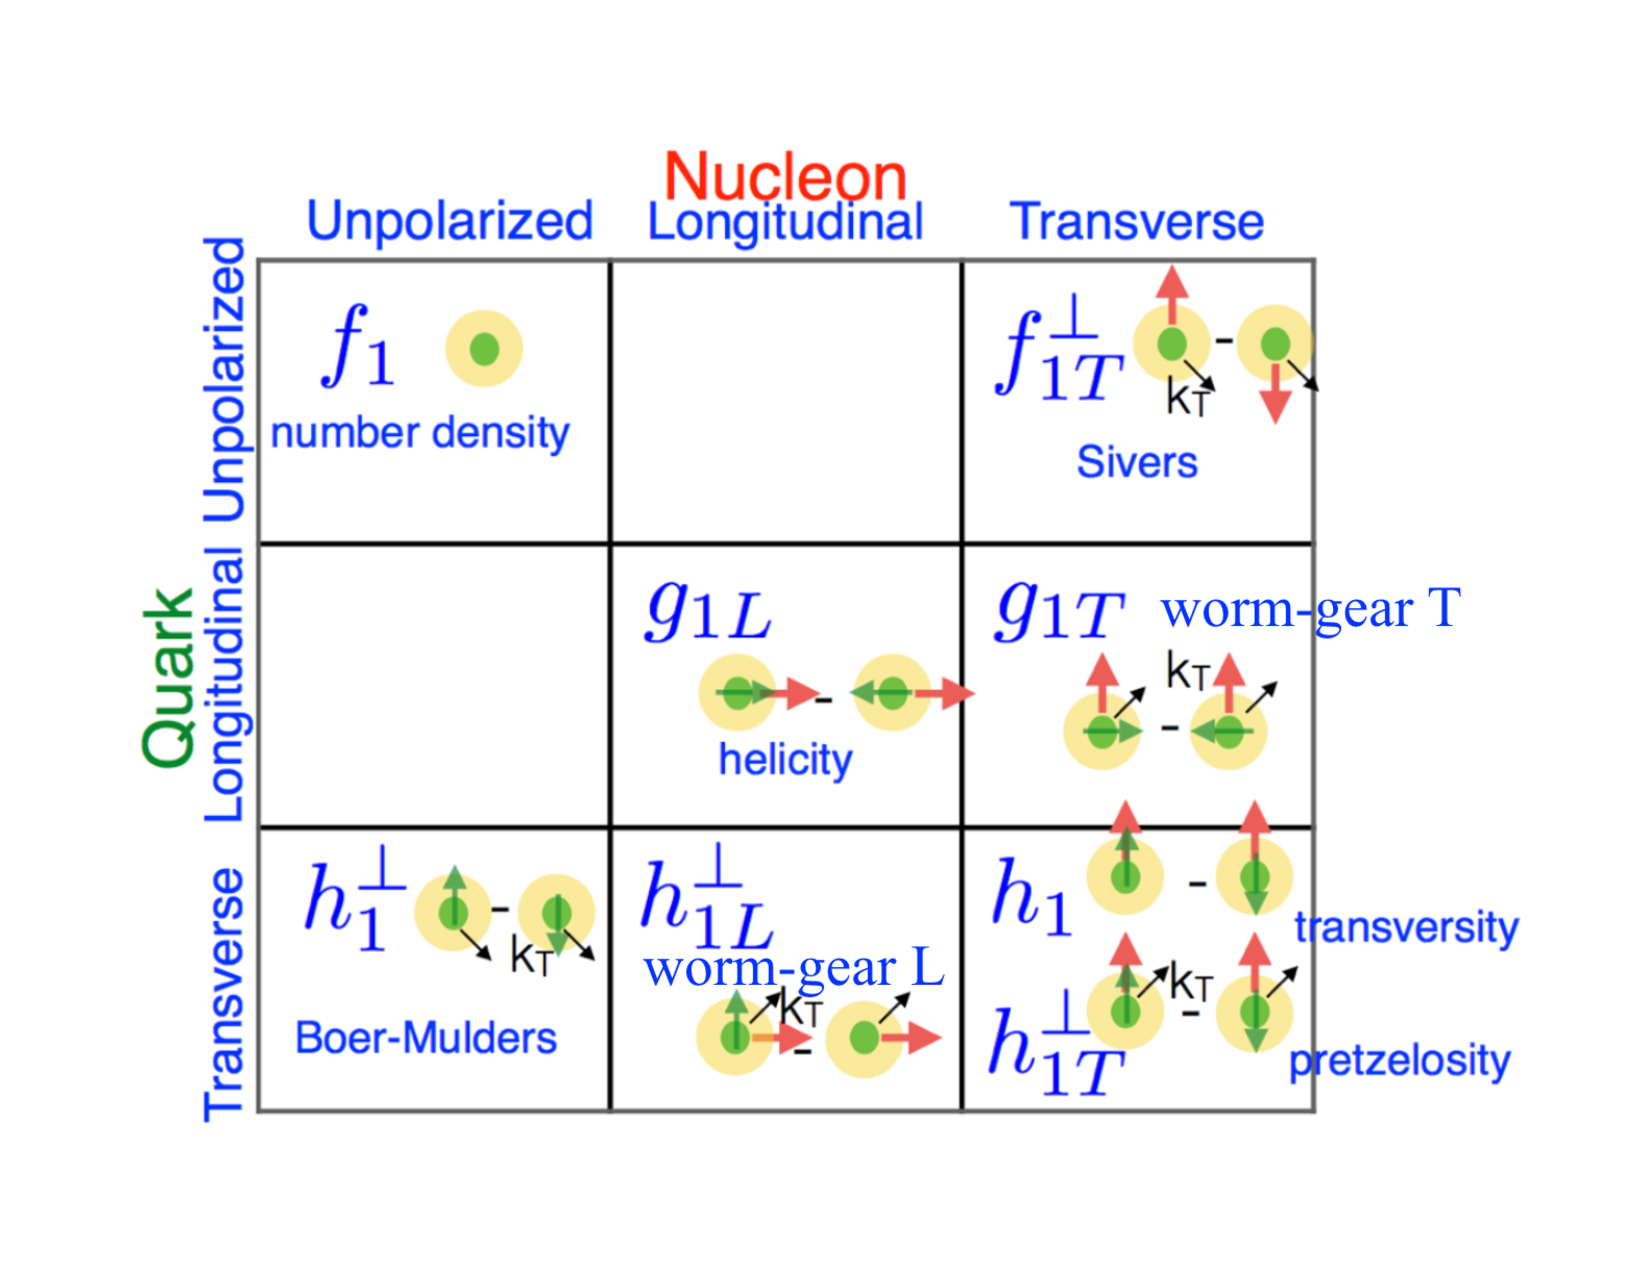
\includegraphics[width=0.6\textwidth, trim=2cm 2cm 2cm 2cm,clip]{TMDs}
  \caption{The eight TMDs needed to describe a spin 1/2 nucleon at leading
    order.  The columns represent the different nucleon polarizations and the
    rows represent the different quark polarizations.  The individual figures
    give a visual representation of the TMD's interpretation.}
  \label{fig::TMDs}
\end{figure}

The TMD functions needed to describe Drell-Yan scattering from a transversely
polarized target, as in the data taking conditions in this thesis are: the
Sivers function, the Boer-Mulders function, the transversity function and the
pretzelosity function.

\subsection{Sivers and Boer-Mulders Distributions}
The Sivers TMD, {\siv}, was first purposed to explain large nucleon
spin-dependent asymmetries~\cite{Sivers}.  The interpretation of the Sivers,
{\siv}, TMD is that it gives a correlation between transverse spin of the parent
hadron and transverse momentum of the scattered parton.  When viewing the hadron
in the direction opposite to it's momentum and using the sign conventions in
this thesis, if {\siv} is positive then it is expected that there are more
partons with momentum pointing left than pointing to the right.  A non-zero
{\siv} then implies that the bound partons in a transversely polarized hadron
are traveling transverse to the hadron's momentum which can intuitively make
senses if the partons have orbital angular momentum.  As of yet however, there
is no theoretical link between orbital angular momentum and the Sivers function.

The Boer-Mulders TMD PDF, $h_1^{\perp}$, was proposed in 1998 as a correlation
between the transverse momentum and the transverse spin of a parton inside an
unpolarized hadron~\cite{Boer:1997nt}.  The Boer-Mulders function is interpreted
as a difference between quarks with transverse momentum and transverse spin up
and quarks with transverse momentum and transverse spin down in an unpolarized
hadron.  It is not hard to realized that changing the chirality of transversely
polarized quarks in an unpolarized hadron would flip the sign of the
Boer-Mulders function which therefore means the Boer-Mulders function is chiral
odd.  Chiral odd functions can only be non-zero when convoluted with another
chiral odd function as is the case when the Boer-Mulders function appears in
either the SIDIS or Drell-Yan cross-section.

The most surprising fact about the Sivers and Boer-Mulders functions is that
they both changes sign under naive time reversal.  Naive time reversal is
defined as reversing time but not swapping initial and final
states~\cite{Bacchetta:2006tn}.  The Sivers and Boer-Mulders functions are
therefore said to be T-odd functions, and as a result, were originally believe
to be forbidden correlations.  However it was shown that the Sivers function
could be non-zero from gluon exchange during the initial state in the Drell-Yan
process and gluon exchange during the final state in the SIDIS
process~\cite{Brodsky:2002cx,Brodsky:2002rv}.  Most surprisingly, it was shown
that a non-zero Sivers function and a non-zero Boer-Mulders function are
expected to have opposite sign in SIDIS and Drell-Yan~\cite{collins_2002}.  That
is

\begin{align}
  f_{1T}^{\bot} |_{Drell-Yan} &= - f_{1T}^{\bot} |_{SIDIS}, \\
  h_{1}^{\bot} |_{Drell-Yan} &= - h_{1}^{\bot} |_{SIDIS}.
\end{align}

\subsection{Transversity and Pretzelosity}
Unlike the Sivers and Boer-Mulders TMDs, the transversity, $h_1(x, k_T)$, and
pretzelosity, $h_{1T}^{\bot}$, TMDs are predicted to be universal functions of a
spin 1/2 hadron.  The transversity is defined for transversely polarized hadrons
as the difference between quarks polarized in the same direction as their parent
hadron and quarks polarized in the opposite direction to their parent hadron.
The transversity distribution is then similar to the helicity distribution,
$g_{1L}$, but for transverse polarizations.  The pretzelosity function is a
correlation between transversely polarized partons and their transverse momentum
in a transversely polarized hadron.  As with the Boer-Mulders TMD, both the
transversity and the pretzelosity TMDs are chiral odd and are therefore
convoluted with another chiral odd function.


\section{Semi-Inclusive Deep Inelastic Scattering} \label{sec::SIDIS}
Semi-Inclusive Deep Inelastic Scattering (SIDIS) is the process where a lepton
scatters electromagnetically off a nucleon and subsequently the scattered lepton
and at least one scattered hadron are detected.  As the name implies, SIDIS is
related to the DIS reaction only SIDIS includes the addition of a detected
hadron.  SIDIS is denoted as

\begin{equation}
  l(\ell, \lambda_l) + N(P, S) \rightarrow l(\ell') + h(P_h) + X(P_X),
\end{equation}
\noindent
where $\lambda_l$ is the helicity of the incoming lepton, $S$ is the spin of the
nucleon, $h$ is the detected hadron and $P_h$ is the detected hadron's four
momentum.  The leading order one photon exchange Feynman diagram for the SIDIS
process is shown in Fig.~\ref{fig::SIDIS_LO}.

\begin{figure}[h!t]
  \centering
  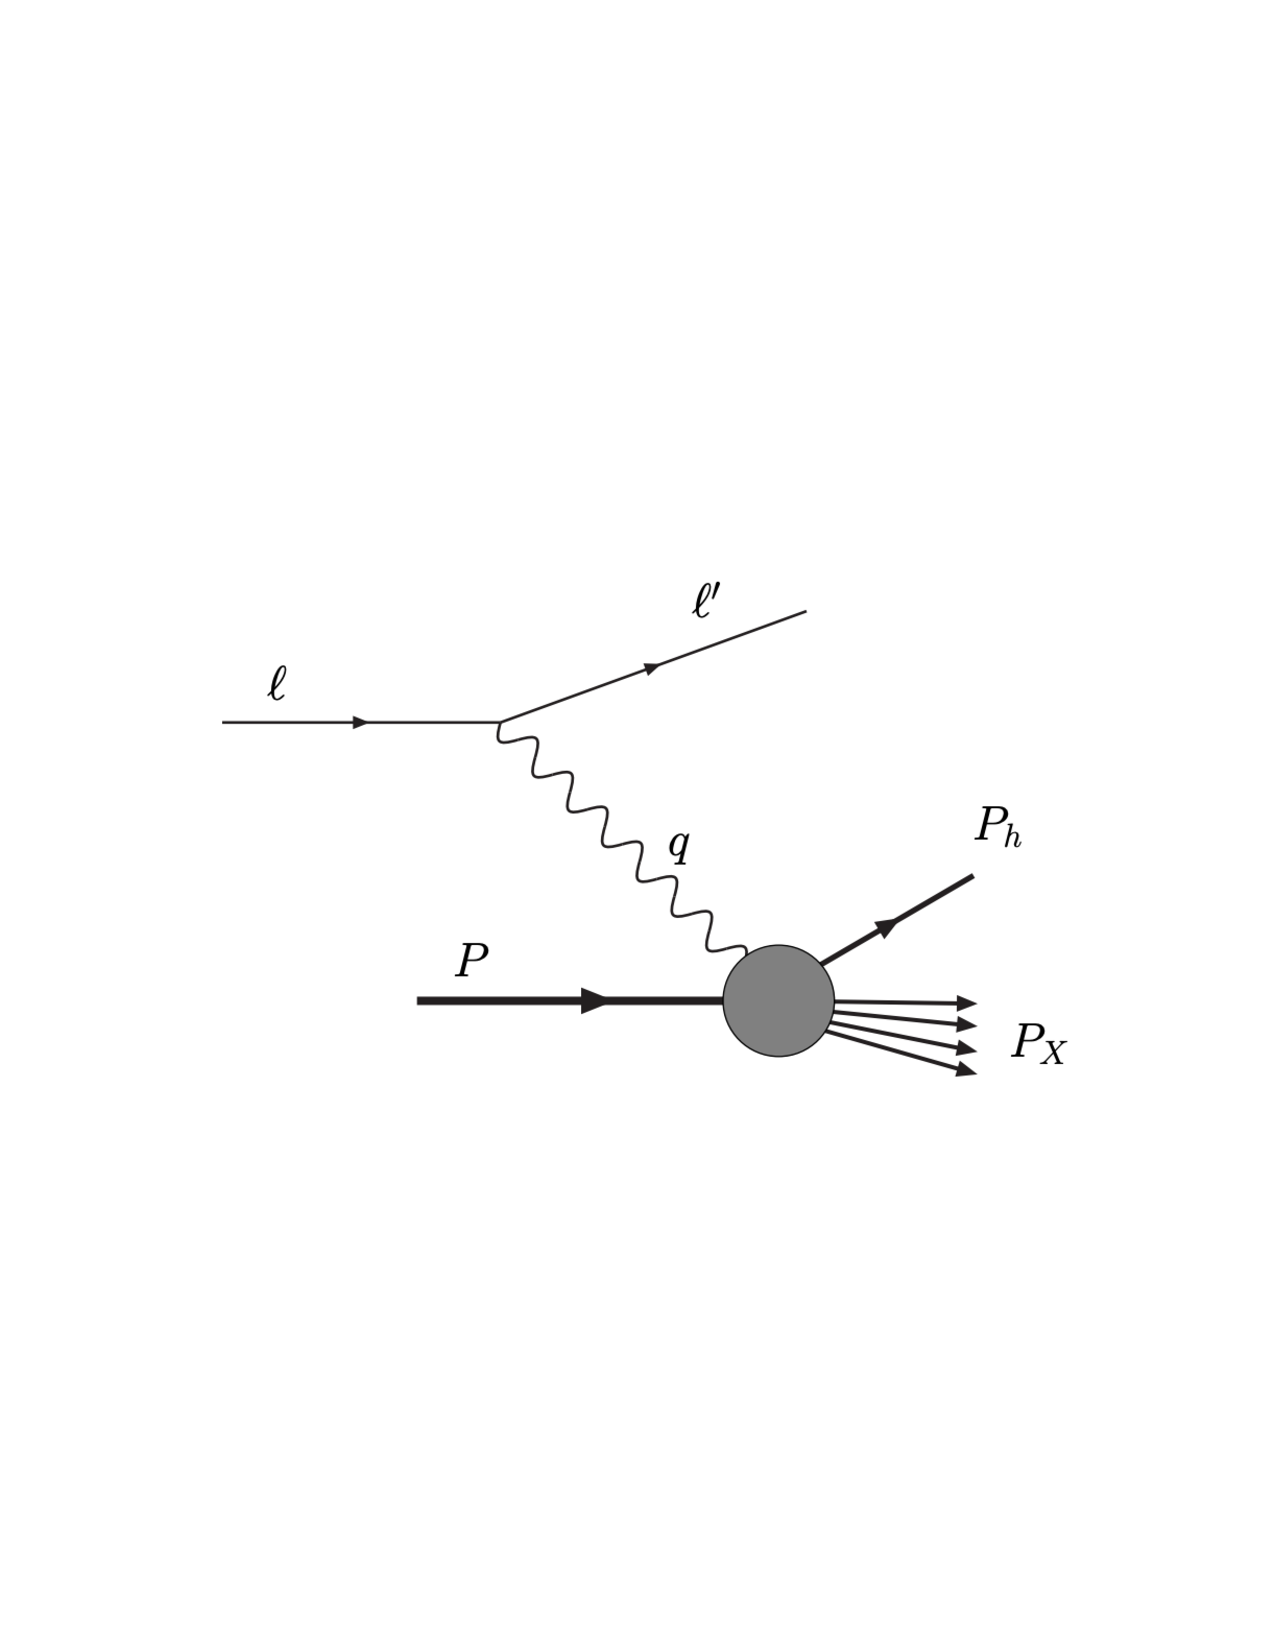
\includegraphics[width=0.5\textwidth, trim=3cm 9cm 3cm 9cm, clip]{SIDIS_LO}
  \caption{The semi-inclusive deep inelastic scattering leading order Feynman
    diagram}
  \label{fig::SIDIS_LO}
\end{figure}

In addition to the kinematic variables used to describe DIS,
Eq.~[\ref{equ::DIS_Q2}-\ref{equ::DIS_W}], one more variable is needed to
describe the SIDIS process,
\begin{equation}
  z = \frac{P \cdot P_h}{P \cdot q} \quad \substack{lab \\frame\\ =} \quad
  \frac{E_h}{E-E'},
\end{equation}
\noindent
which is interpreted as the fraction of possible energy the detected hadron
can obtain.  The transverse spin-dependent SIDIS cross-section can be described
in a model independent way using structure functions as~\cite{Bacchetta:2006tn}

\begin{align}
  \frac{d\sigma}{dx \, dy\, d\psi \,dz\, d\phi_h\, d P_{h\perp}^2} &=
  \frac{\alpha^2}{x y Q^2}\,
  \frac{y^2}{2\,(1-\varepsilon)}\,  \biggl( 1+\frac{\gamma^2}{2x} \biggr)\,
  \Biggl\{
  F_{UU ,T}
  + 
  \varepsilon
  F_{UU ,L}
  + \sqrt{2\,\varepsilon (1+\varepsilon)}\,\cos\phi_h\,
  F_{UU}^{\cos\phi_h}
  \nonumber \\  & 
  + \varepsilon \cos(2\phi_h)\, 
  F_{UU}^{\cos 2\phi_h}
  + \lambda_l\, \sqrt{2\,\varepsilon (1-\varepsilon)}\, 
  \sin\phi_h\, 
  F_{LU}^{\sin\phi_h}
  \phantom{\Bigg[ \Bigg] }
  \nonumber \\  & 
  + |S_\perp|\, \Bigg[
    \sin(\phi_h-\phi_S)\,
    \Bigl(F_{UT ,T}^{\sin\left(\phi_h -\phi_S\right)}
    + \varepsilon\, F_{UT ,L}^{\sin\left(\phi_h -\phi_S\right)}\Bigr)
    \nonumber \\  & \quad  \qquad \qquad
    + \varepsilon\, \sin(\phi_h+\phi_S)\, 
    F_{UT}^{\sin\left(\phi_h +\phi_S\right)}
    + \varepsilon\, \sin(3\phi_h-\phi_S)\,
    F_{UT}^{\sin\left(3\phi_h -\phi_S\right)}
    \phantom{\Bigg[ \Bigg] }
    \nonumber \\  & \quad \qquad \qquad
    + \sqrt{2\,\varepsilon (1+\varepsilon)}\, 
    \sin\phi_S\, 
    F_{UT}^{\sin \phi_S }
    + \sqrt{2\,\varepsilon (1+\varepsilon)}\, 
    \sin(2\phi_h-\phi_S)\,  
    F_{UT}^{\sin\left(2\phi_h -\phi_S\right)}
    \Bigg]
  \nonumber \\  &
  + |S_\perp| \lambda_l\, \Bigg[
    \sqrt{1-\varepsilon^2}\, \cos(\phi_h-\phi_S)\, 
    F_{LT}^{\cos(\phi_h -\phi_S)}
    +\sqrt{2\,\varepsilon (1-\varepsilon)}\, 
    \cos\phi_S\, 
    F_{LT}^{\cos \phi_S}
    \nonumber \\  & \quad \qquad \qquad
    +\sqrt{2\,\varepsilon (1-\varepsilon)}\, 
    \cos(2\phi_h-\phi_S)\,  
    F_{LT}^{\cos(2\phi_h - \phi_S)}
    \Bigg] \Biggr\},
  \label{equ::SIDISxsect}
\end{align}
\noindent
where
\begin{equation}
  \varepsilon =
  \frac{1-y-\frac{1}{4}\gamma^2y^2}{1-y+\frac{1}{2}y^2+\frac{1}{4}\gamma^2y^2},
\end{equation}
\noindent
and $\gamma = \frac{2Mx}{Q}$, $\psi$ is the azimuthal scattering angle of the
lepton around the lepton beam with respect to the transverse spin direction of
the target and where this cross-section is defined in the $\gamma$-nucleon
reference frame.  The $\gamma$-nucleon reference system is a lab frame where
the virtual photon is along the z-axis and the xz-plane is determined by the
lepton plane.  Fig.~\ref{fig::gammaNucleonFrame} shows the $\gamma$-nucleon lab
frame and the relevant azimuthal angles.

\begin{figure}[h!t]
  \centering 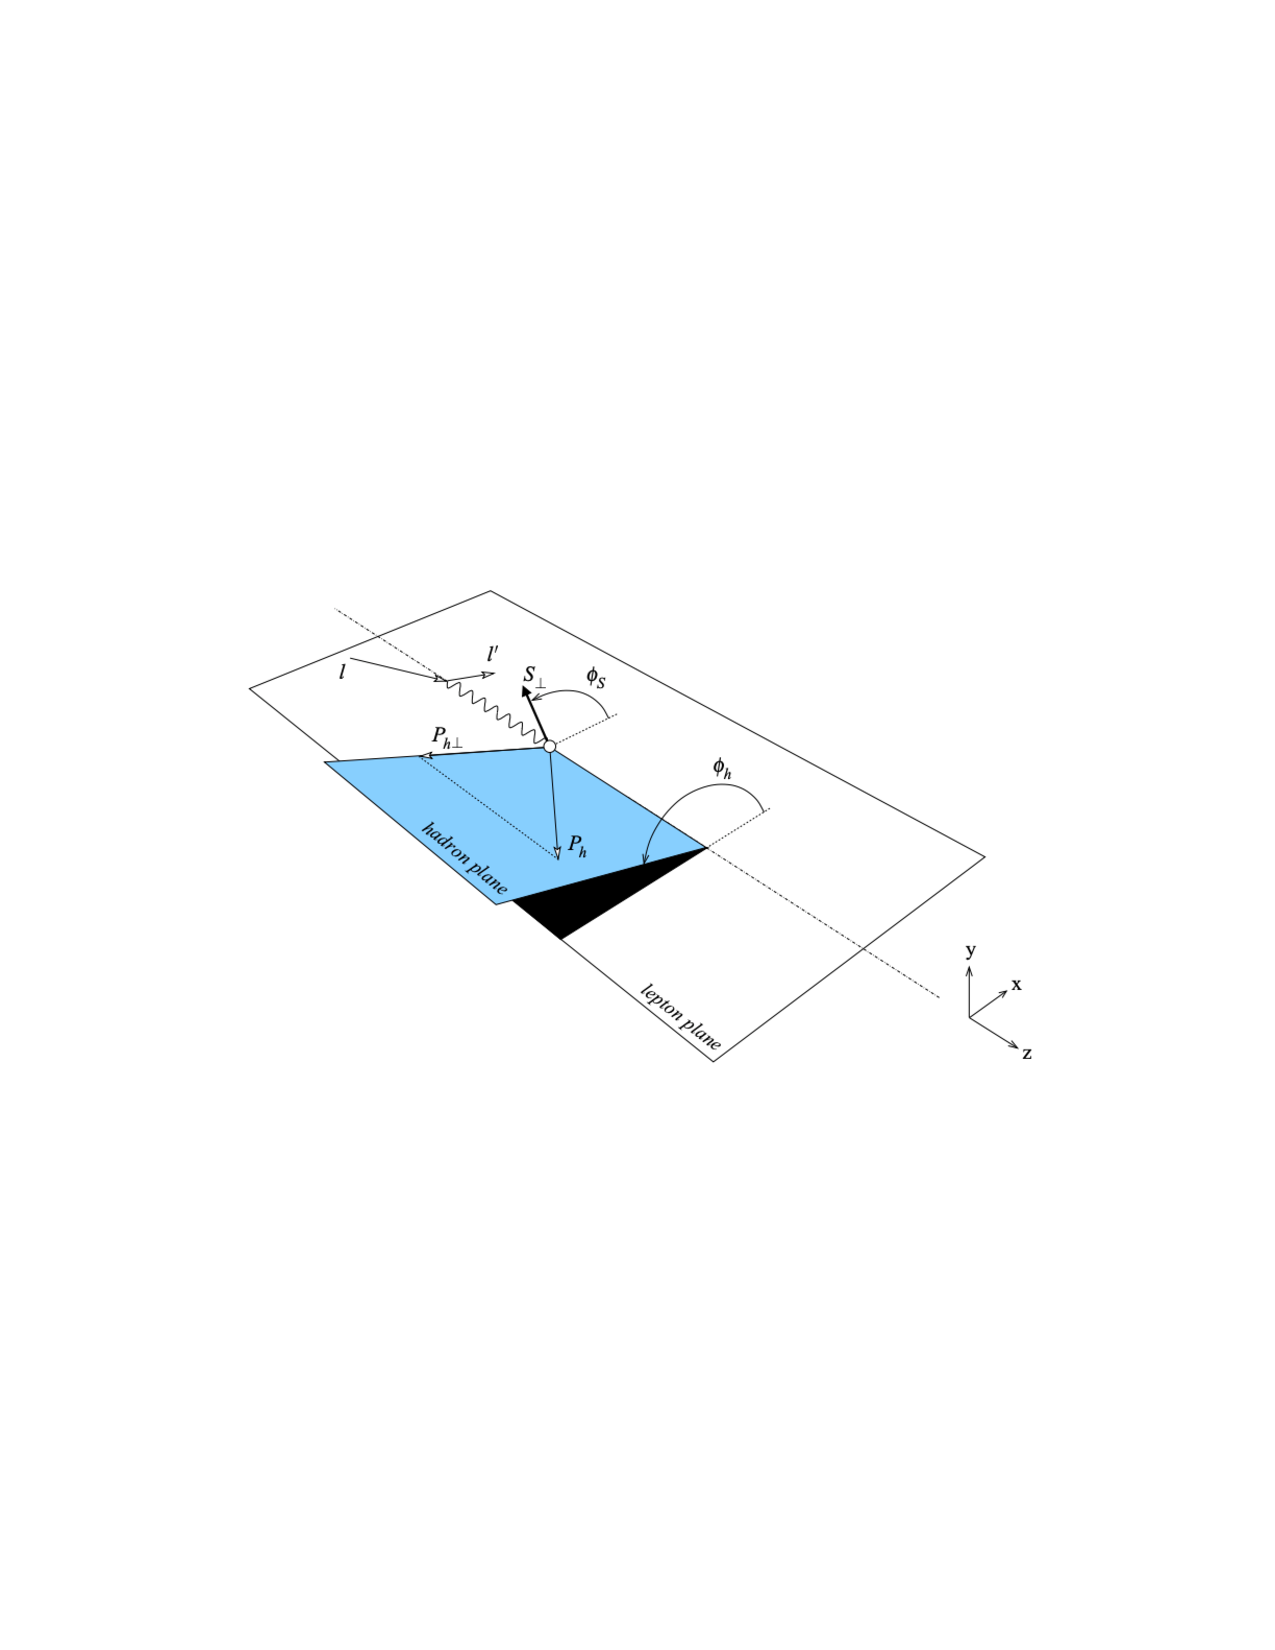
\includegraphics[width=0.6\textwidth,trim=3cm 9cm 3cm 8cm,
    clip]{gammaNucleonFrame}
  \caption{The $\gamma$-nucleon lab frame where the target nucleon is at rest
    and the virtual photon is along the z-axis.  The lepton scattering plane
    defines the xz-plane where the outgoing lepton defines the positive
    x-direction.  This image was taken from~\cite{Bacchetta:2006tn}.}
  \label{fig::gammaNucleonFrame}
\end{figure}

The 14 structure functions in Eq.~\ref{equ::SIDISxsect} are coefficients to the
azimuthal angles from the $\gamma$-nucleon reference frame.  The structure
functions are label as $F$ where the superscript denotes which azimuthal angle
coefficient they correspond to and the three subscripts represent the beam,
target and virtual photon polarization from left to right respectively.  The
subscript polarizations are $U$ for unpolarized, $L$ for longitudinally
polarized and $T$ for transversely polarized.  The cross-section,
Eq.~\ref{equ::SIDISxsect}, is determined similarly to the DIS
cross-section, Eq.~\ref{equ::DIS_diffxsection}, in that structure functions are
used to generically parameterize the hadronic tensor.

In the TMD regime the structure functions are related to TMD functions and
fragmentation functions (FF).  For SIDIS, the TMD regime is defined as the
detected hadron's transverse momentum being small compared to the virtual photon
momentum, $P_{hT} << Q$.  Then in this regime the model independent structure
functions are equal to a convolution of a TMD and a FF where the
convolution is defined as

\begin{equation}
  \label{equ::SIDIS_conv}
{\cal C}\bigl[ w(p_T,k_T) f D \bigr] = x \sum_q e_q^2 \int d^2 p_T d^2 k_T
\delta^{(2)}\bigl(p_T - k_T - P_{h \perp}/z \bigr) w(p_T,k_T)
f^q(x,p_T^2)D^q(z,k_T^2),
\end{equation}
\noindent
where $w$ is a weight $f$ is a TMD function and $D$ is a FF.  For the structure
functions related to transverse target polarization, the relations between
structure functions and TMDs at leading order are~\cite{Bacchetta:2006tn}

\begin{align}
  \label{equ::F_UUTsinphihphis}
  F_{UT ,T}^{\sin\left(\phi_h -\phi_S\right)} &=
  {\cal C}\biggl[-\frac{\hat{h} \cdot p_T}{M} f_{1T}^{\perp } D_1\biggr]
  &\propto f_{1T}^{\perp } \otimes D_1, \\
  F_{UT ,L}^{\sin\left(\phi_h -\phi_S\right)} &= 0,\\
  F_{UT}^{\sin(\phi_h +\phi_S)} &=
  {\cal C}\biggl[-\frac{\hat{h}\cdot k_T^{}}{M_h} h_{1} H_1^{\perp }\biggr]
  &\propto h_{1} \otimes H_1^{\perp },\\
  F_{UT}^{\sin(3\phi_h -\phi_S)} &=
  {\cal C}\biggl[ \frac{2 \bigl(\hat{h}\cdot
      p_T \bigr) \bigl( \bm{p}_T\cdot k_T^{} \bigr) +\bm{p}_T^2
      \bigl(\hat{h}\cdot k_T^{} \bigr) -4 (\hat{h}\cdot p_T)^2 (\hat{h}\cdot
      k_T^{})}{2 M^2 M_h} h_{1T}^{\perp } H_1^{\perp }\biggr]
  &\propto h_{1T}^{\perp } \otimes H_1^{\perp },\\
  \label{equ::F_LTcosphihphis}
  F_{LT}^{\cos(\phi_h -\phi_S)}
  &={\cal C}\biggl[ \frac{\hat{h} \cdot p_T}{M} g_{1T}
    D_1 \biggr]
  &\propto g_{1T} \otimes D_1, 
\end{align}

\noindent
and the leading order structure functions related to an unpolarized target are

\begin{align}
  F_{UU ,T} &= {\cal C}\bigl[ f_1 D_1 \bigr] &\propto f_1 \otimes D_1, \\
  \label{equ::F_UUL}
  F_{UU ,L} &= 0 \\
  \label{equ::F_UUcos2phi}
  F_{UU}^{\cos 2\phi_h} &= {\cal C}\biggl[
   - \frac{2 \bigl( \hat{h} \cdot k_T \bigr)
     \bigl( \hat{h} \cdot p_T \bigr)
     -k_T^{} \cdot p_T}{M M_h}
   h_{1}^{\perp } H_{1}^{\perp }\biggr]
  &\propto h_1^{\perp} \otimes H_1^{\perp}, 
\end{align}

\noindent
where the unit vector $\hat{h}=P_{h \perp}/|P_{h\perp}|$ and $D_1$ and
$H_1^{\perp}$ are fragmentation functions.

The fragmentation functions are functions of $z$ and describe the probability
for a quark to hadronize to a specific hadron.  These fragmentation functions
depend on the quark spin, the hadron type and polarization, and the quark $k_T$.
In Eq.~[\ref{equ::F_UUTsinphihphis}-~\ref{equ::F_UUL}] the fragmentation
function $D_1$ refers to an unpolarized quark fragmenting to an unpolarized
hadron and $H_1^{\perp}$ refers to a transversely polarized quark fragmenting to
an unpolarized hadron.

The SIDIS cross-section, Eq.~\ref{equ::SIDISxsect}, can be rewritten in terms of
asymmetries.  These asymmetries are defined as

\begin{equation}
  A^{w_i(\phi_h, \phi_S)}_{BeamTarget} = \frac{F^{w_i(\phi_h,
      \phi_S)}_{BeamTarget}}{F_{UU,T}+\varepsilon F_{UU,L}},
  \label{equ::asymAmpSIDIS}
\end{equation}
\noindent
where $w_i(\phi_h, \phi_S)$ is the azimuthal angle associated with this
asymmetry and $Beam$ and $Target$ represent the polarization of the beam and
target.  The asymmetry amplitude, Eq.~\ref{equ::asymAmpSIDIS}, is a structure
function divide by the unpolarized structure functions.  This asymmetry
amplitude definition is defined because it is easier to measure experimentally.
In order to determine an asymmetry amplitudes, the number of counts
experimentally measured are fit using a function in the form of
Eq.~\ref{equ::SIDISxsect}.  The parameters of this fit are the coefficients to
each azimuthal amplitude.  The results of the fit can then determine the
spin-dependent asymmetry amplitudes without needing to determine luminosity and
therefore have reduced systematic errors.

\subsection{SIDIS TMD Results}
COMPASS and HERMES measuremented the asymmetry $A_{UT ,T}^{\sin\left(\phi_h
  -\phi_S\right)}$ from the SIDIS reaction from a transversely polarized proton
target~\cite{Alekseev:2008aa,Airapetian:2009ae}.  The comparison of the results
between these two collaborations is shown in Fig.~\ref{fig::SiversFromSIDIS}.
The asymmetry amplitude $A_{UT ,T}^{\sin\left(\phi_h-\phi_S\right)}$ is related
to the Sivers function and was measured to be non-zero at a level up to 5\%.

\begin{figure}[h!t]
  \centering 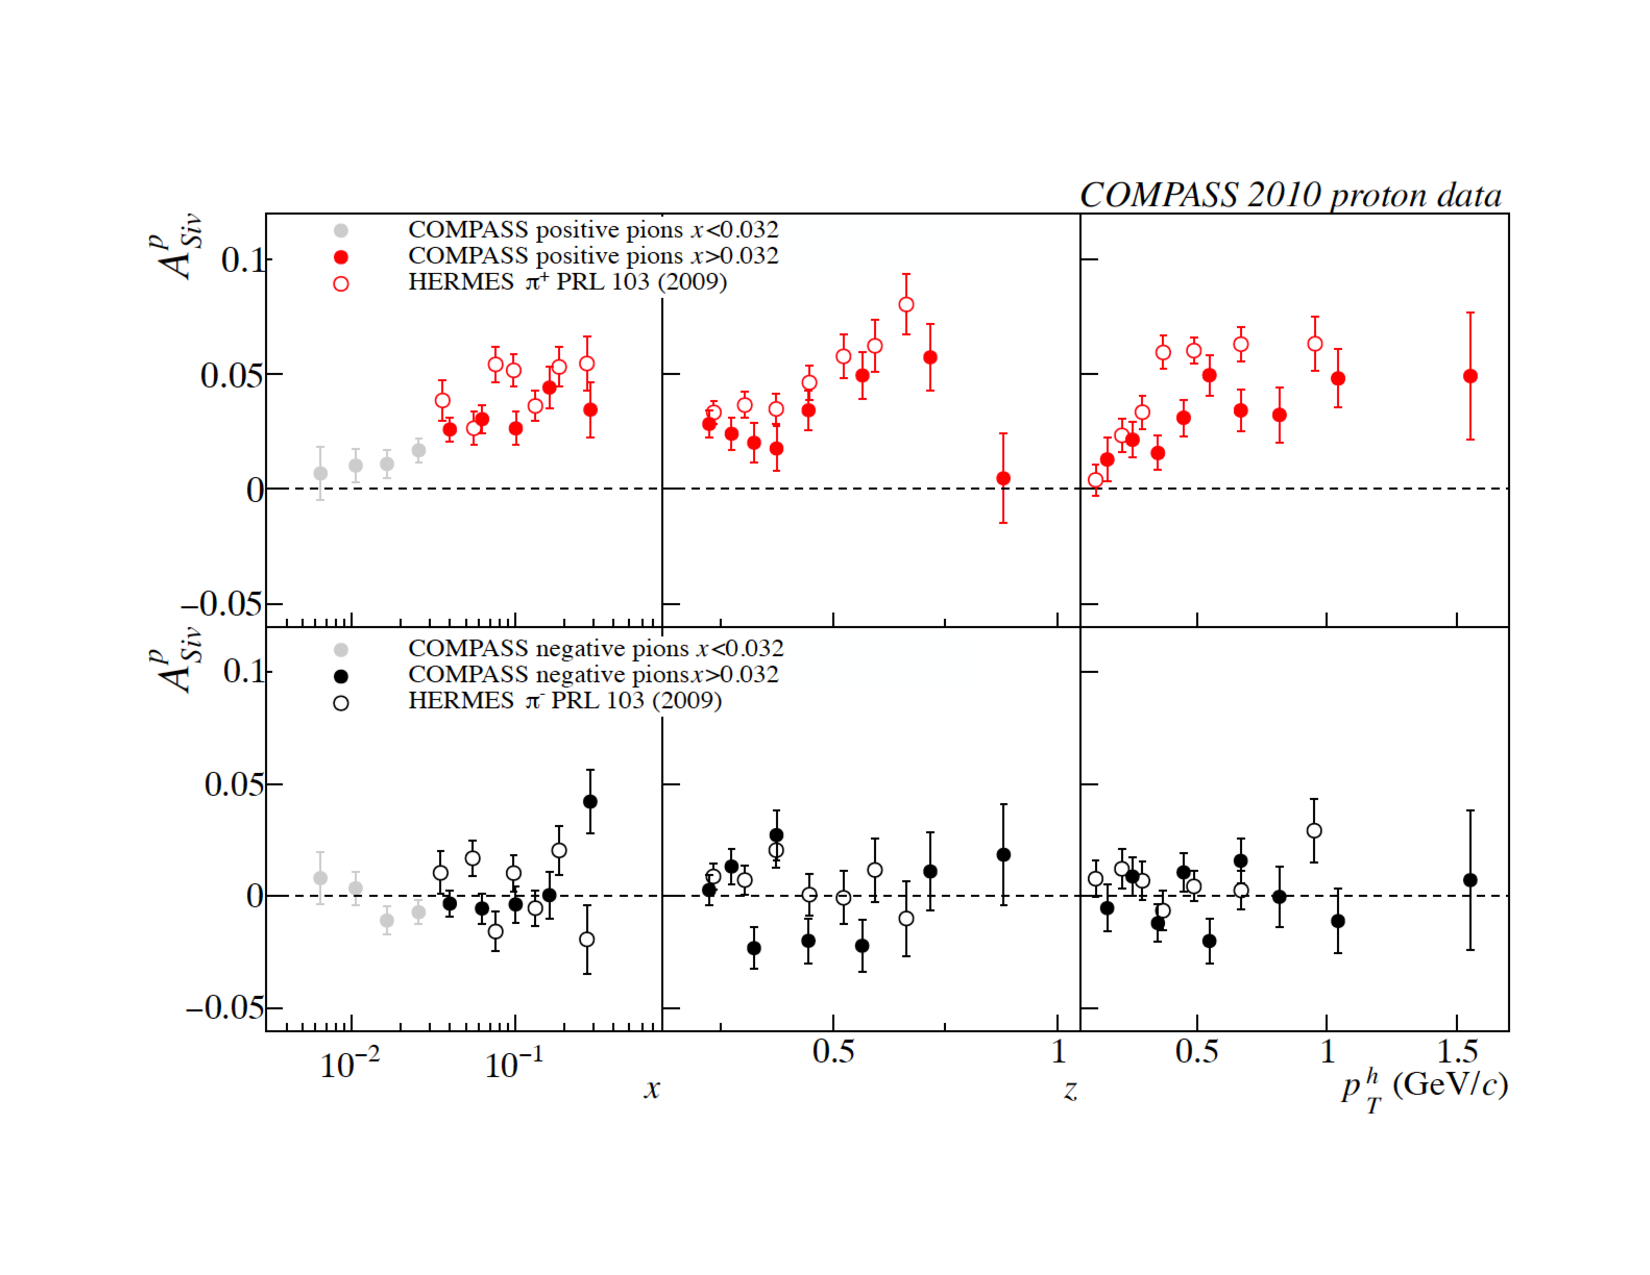
\includegraphics[width=0.6\textwidth, trim=2cm 2cm 2cm
    3cm,clip]{SiversFromSIDIS}
  \caption{The asymmetry amplitude related to the Sivers function measure by
    COMPASS~\cite{Alekseev:2008aa} and HERMES~\cite{Airapetian:2009ae}}
  \label{fig::SiversFromSIDIS}
\end{figure}

The top plot in Fig.~\ref{fig::SiversFromSIDIS} is the asymmetry for a positive
detected hadron.  A positively detected final state hadron is dominated by
u-quark scattering and therefore by the u-quark Sivers function.  This is the
case for three reasons.  Firstly because the SIDIS reaction is weighted by
$e_q^2$ which therefore makes the u-quark scattering four times more likely.
Secondly the so-called favored FF, where the detected hadron is the same charge
as the quark which fragmented, is larger than the unfavored FF.  Therefore a
positively detected hadron most likely resulted from a positively fragmenting
quark.  Thirdly the proton target is composed of twice as many u-quarks as
d-quarks in this scattering kinematic region.  For these three reasons the
results in Fig.~\ref{fig::SiversFromSIDIS} imply that the u-quark Sivers
function from the SIDIS reaction is positive.

The bottom plots in Fig.~\ref{fig::SiversFromSIDIS} suggest that the d-quark
Sivers function in the SIDIS reaction is negative.  The bottom results in
Fig.~\ref{fig::SiversFromSIDIS} are from the combination of u-quark scattering
and fragmenting unfavoredly and d-quark scattering and fragmenting favoredly.
As was mentioned the charge weighting in the SIDIS reaction and the proton quark
composition results in the u-quark scattering with a higher probability.  On the
other hand the previous effect is canceled out by the fact that the favor FF for
the d-quark fragmenting is larger than the unfavored FF for the u-quark
fragmenting.  Therefore the results in the bottom of
Fig.~\ref{fig::SiversFromSIDIS} are for an approximately equal combination from
u-quark scattering and d-quark scattering.  As the u-quark asymmetry amplitude
is positive, the d-quark asymmetry amplitude must therefore be negative and so
also must the d-quark Sivers function.  Anselmino et. al. extracted the Sivers
function using both HERMES and COMPASS data and additional data for
fragmentation functions~\cite{PhysRevD.86.014028}.  These results are shown in
Fig.~\ref{fig::SiversExtractedFromSIDIS}.

\begin{figure}[h!t]
  \centering 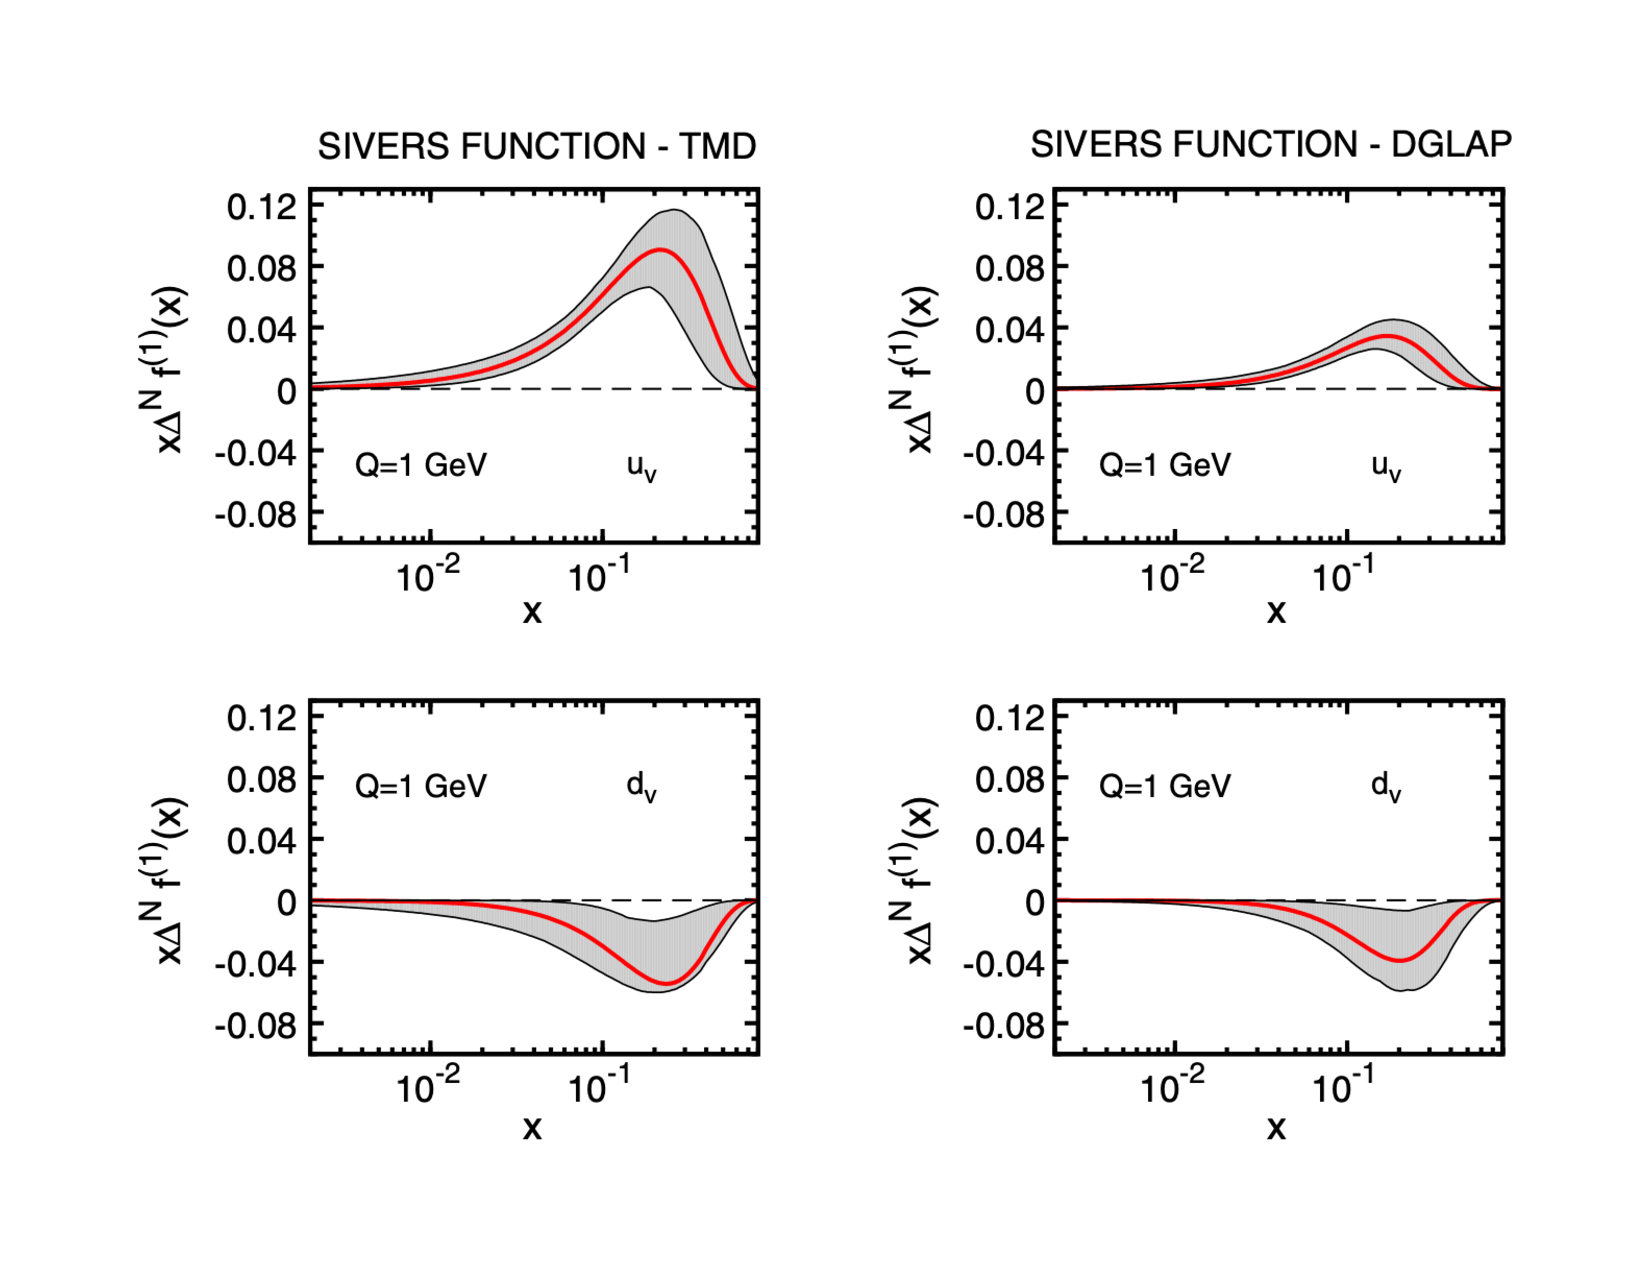
\includegraphics[width=0.6\textwidth, trim=2cm 2cm 2cm 2cm,
    clip]{SiversExtractedFromSIDIS}
  \caption{The valence quark distributions for the first moment of the Sivers
    function.  The left plots are using TMD evolution and the right plots are
    using DGLAP evolution to globally include all measured data.  This image was
    taken from~\cite{PhysRevD.86.014028}}
  \label{fig::SiversExtractedFromSIDIS}
\end{figure}

Results for the TMD asymmetry amplitude, $A_{UU}^{\cos 2\phi_h}$, related to the
Boer-Mulders function were measured by the COMPASS collaboration from
SIDIS~\cite{Adolph:2014pwc}.  As can be seen from the convolution of the
structure function, Eq.~\ref{equ::F_UUcos2phi}, and the definition of asymmetry
amplitudes in SIDIS, Eq.~\ref{equ::asymAmpSIDIS}, this asymmetry amplitude is a
convolution of the Boer-Mulders function and a fragmentation function.  The
COMPASS results for $A_{UU}^{\cos 2\phi_h}$ are shown in
Fig.~\ref{fig::BMFromSIDIS}.  Notably the Boer-Mulders asymmetry amplitude is
higher for negatively scattered hadrons than for positively scattered hadrons
suggesting that the Boer-Mulders function is larger for d-quarks than for
u-quarks.

\begin{figure}[h!t]
  \centering
  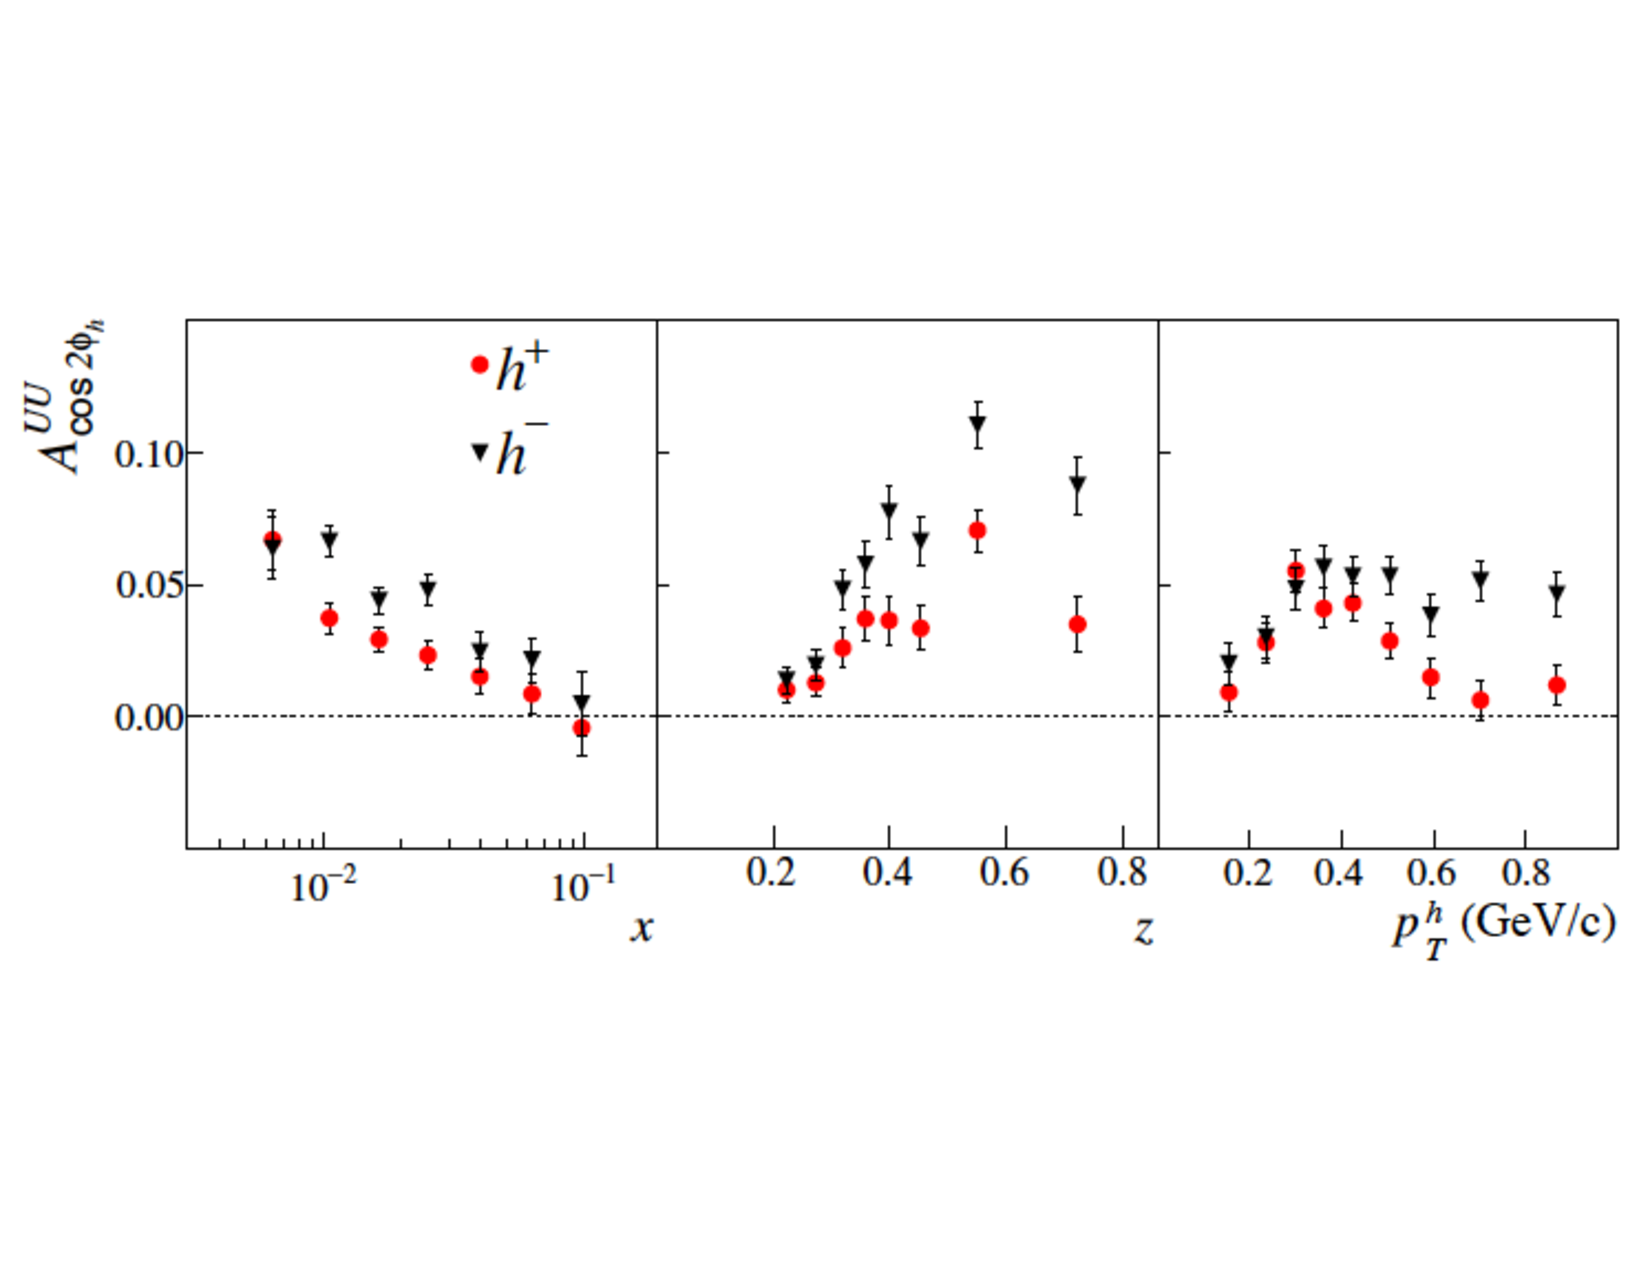
\includegraphics[width=0.7\textwidth,trim=0.3cm 5cm 0cm 4cm,clip]{BMFromSIDIS}
  \caption{COMPASS SIDIS data from muons scattered off of a deuteron target for
    positively scatted hadrons (red) and negatively scattered hadrons (black).
    The asymmetry amplitude is related to the Boer-Mulders functions.  This
    image was taken from~\cite{Adolph:2014pwc}}
  \label{fig::BMFromSIDIS}
\end{figure}

Three SIDIS experiments measured data related to the transversity distribution
from the structure function $F_{UT}^{\sin(\phi_h +\phi_S)}$.  These three
experiments were HERMES~\cite{Airapetian:2004tw,Airapetian:2010ds},
COMPASS~\cite{Ageev:2006da,Alekseev:2008aa,Alekseev:2010rw,Adolph:2012sn,Adolph:2014zba},
and JLab HALL A~\cite{PhysRevLett.107.072003}.  The FF data to determine
$H_1^{\perp }$ from the structure function, $F_{UT}^{\sin(\phi_h +\phi_S)}$,
comes from BELLE~\cite{Abe:2005zx,Seidl:2008xc} and
BABAR~\cite{TheBABAR:2013yha} data in $e^+e^-$ annihilation data.  Anselmino et. al. extracted the transversity distribution~\cite{PhysRevD.87.094019} from
all this data and their results are shown in
Fig.~\ref{fig::transversityExtractedFromSIDIS}.

\begin{figure}[h!t]
  \centering 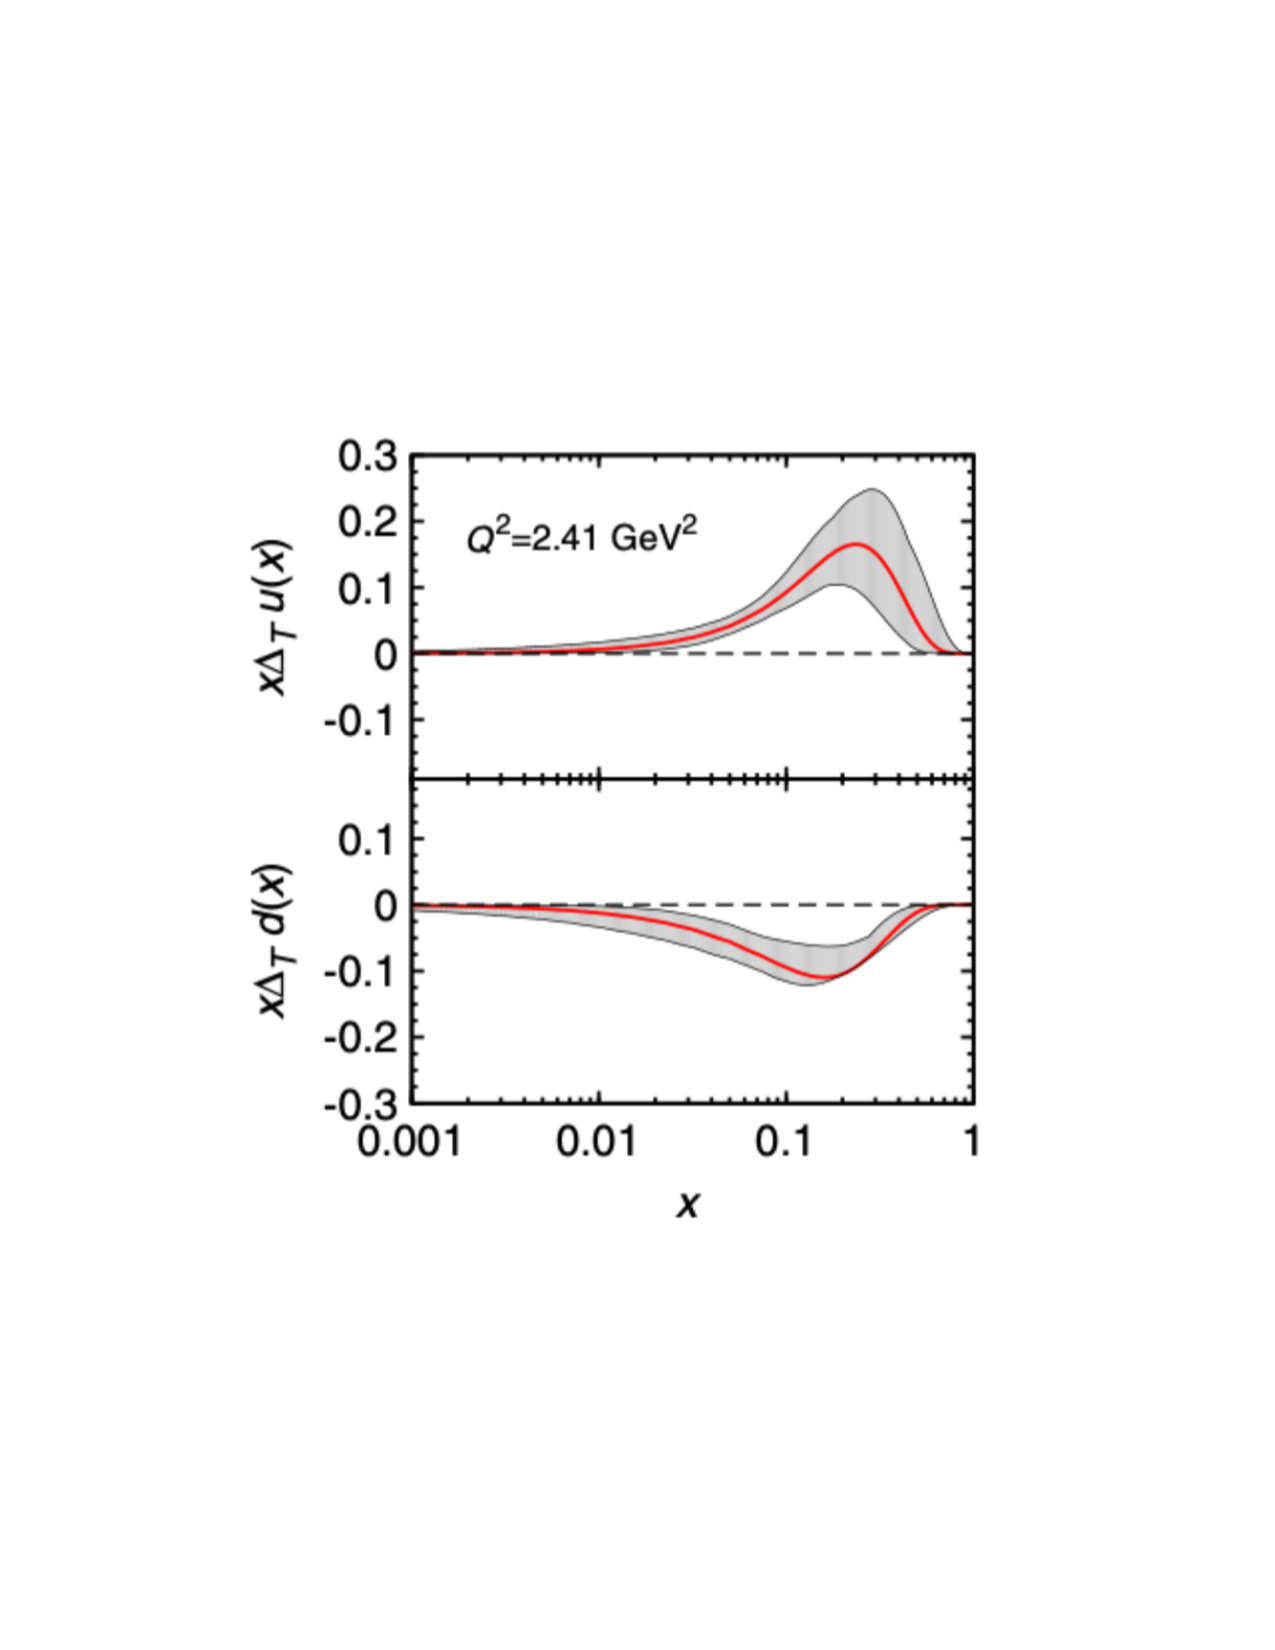
\includegraphics[width=0.4\textwidth, trim=4cm 7cm 4cm 6cm,
    clip]{transversityExtractedFromSIDIS}
  \caption{The transversity distribution for u-quarks (top) and d-quarks
    (bottom) determined from SIDIS data and $e^+e^-$ data.  Image taken
    from~\cite{PhysRevD.87.094019}.}
  \label{fig::transversityExtractedFromSIDIS}
\end{figure}


\section{Drell-Yan} \label{sec::DY}
The Drell-Yan process is the reaction where a quark and an anti-quark annihilate
and the end product results in two detected leptons.  The Drell-Yan process is
denoted as

\begin{equation}
  H_a(P_a) + H_b(P_b, S) \rightarrow \gamma^* + X \rightarrow l(\ell) +
  l'(\ell') + X
\end{equation}
\noindent
where $H_a$ and $H_b$ are hadrons which carry the quark and anti-quarks and in
this thesis only the target hadron, $H_b$ is considered to be polarized with
spin $S$.  In this thesis the quark and anti-quark pair annihilate to form a
virtual photon, $\gamma^*$ and additionally the only final state detected
leptons considered are a muon and an anti-muon pair.  The leading order one
photon exchange diagram is shown in Fig.~\ref{fig::DY_LO}.

\begin{figure}[h!t]
  \centering
  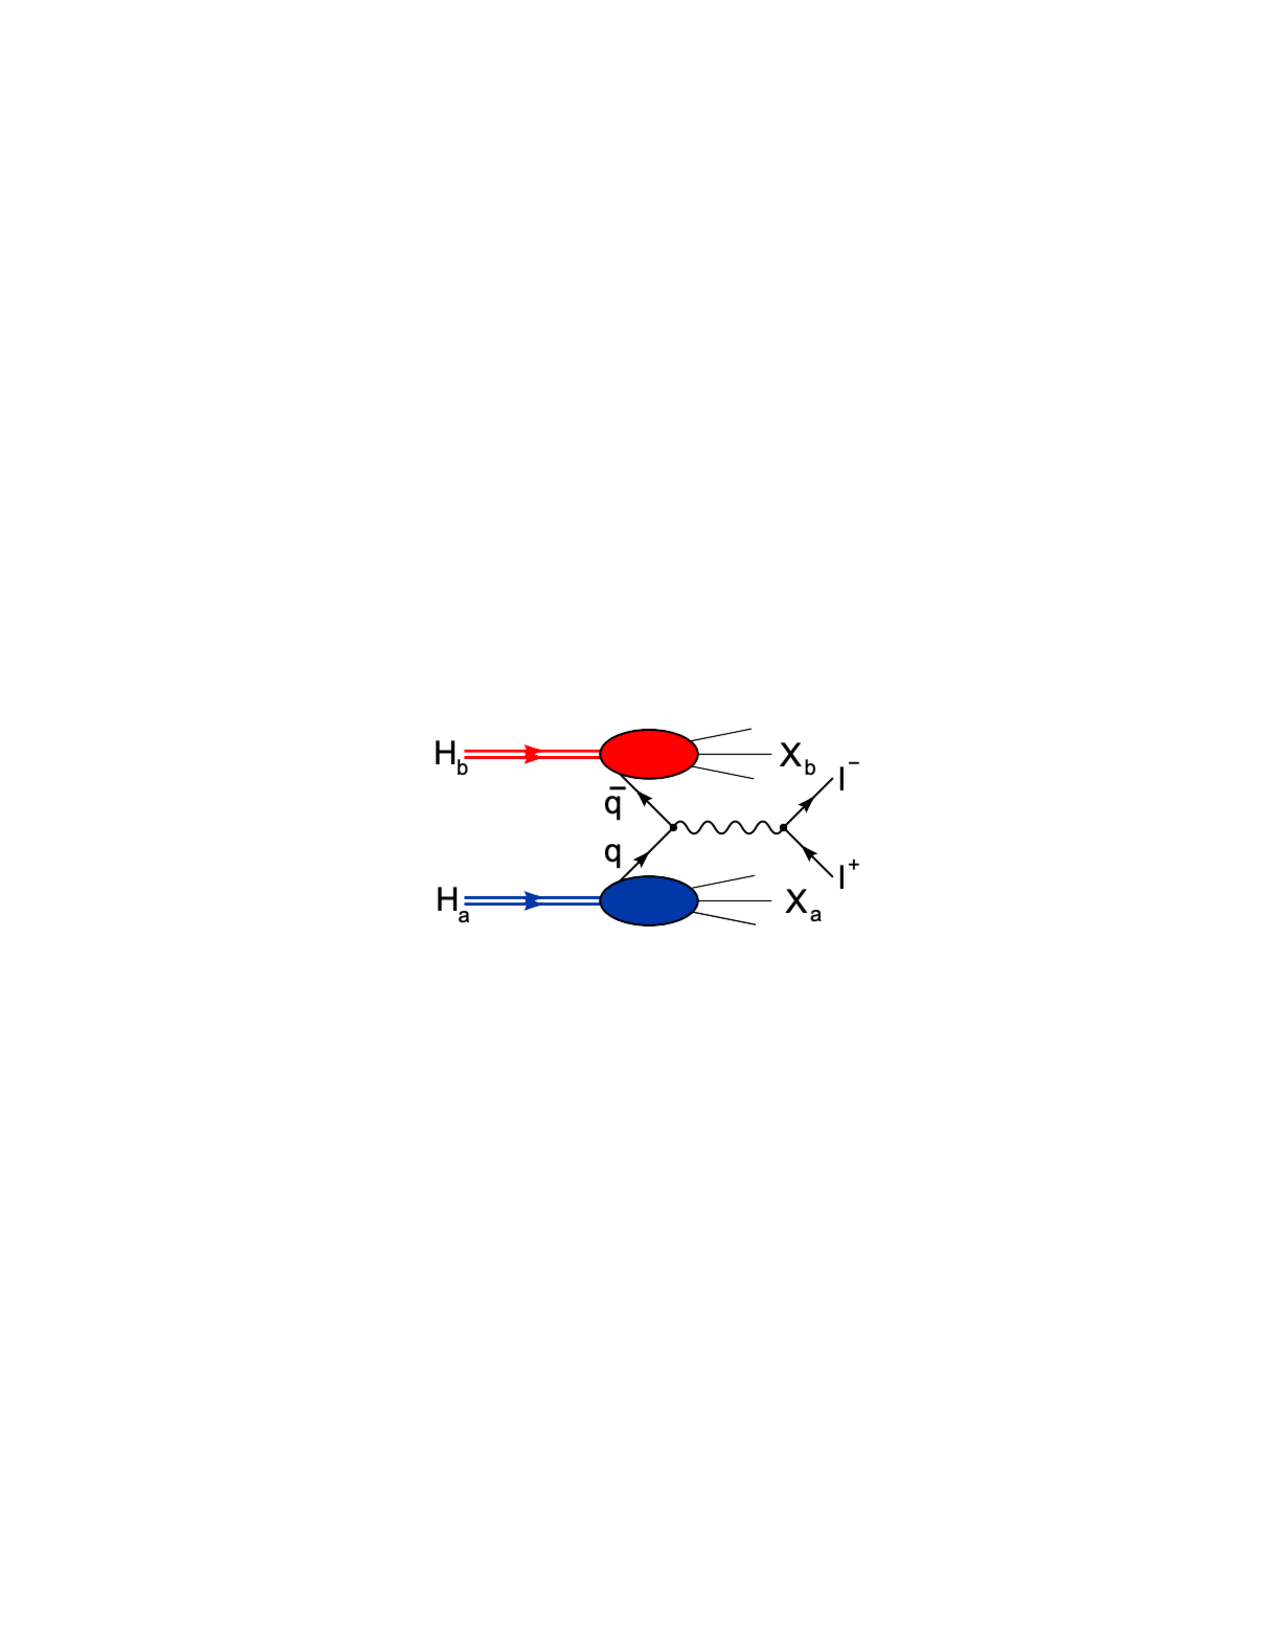
\includegraphics[width=0.45\textwidth, trim=7cm 12cm 7cm 12cm, clip]{DY_LO}
  \caption{The Drell-Yan leading order diagram}
  \label{fig::DY_LO}
\end{figure}

The angles used to define the general Drell-Yan cross-section are defined with
the use of two reference frames.  The target frame (TF),
Fig.~\ref{fig::DY_TargetFrame}, defines the $\phi_S$ angle and the Collins-Soper
(CS), Fig.~\ref{fig::DY_CSFrame}, frame defines the additional $\phi$ and
$\theta$ angles.  The $\phi_S$ angle is defined in the TF as the angle between
the transverse momentum of the virtual photon and the transverse spin of the
target.  The $\phi$ and $\theta$ angles, in the CS frame, are defined as the
azimuthal and polar angle of the negatively charged muon.

\begin{figure}[h!t]
  \centering
  \begin{subfigure}{.46\textwidth}
    \centering
    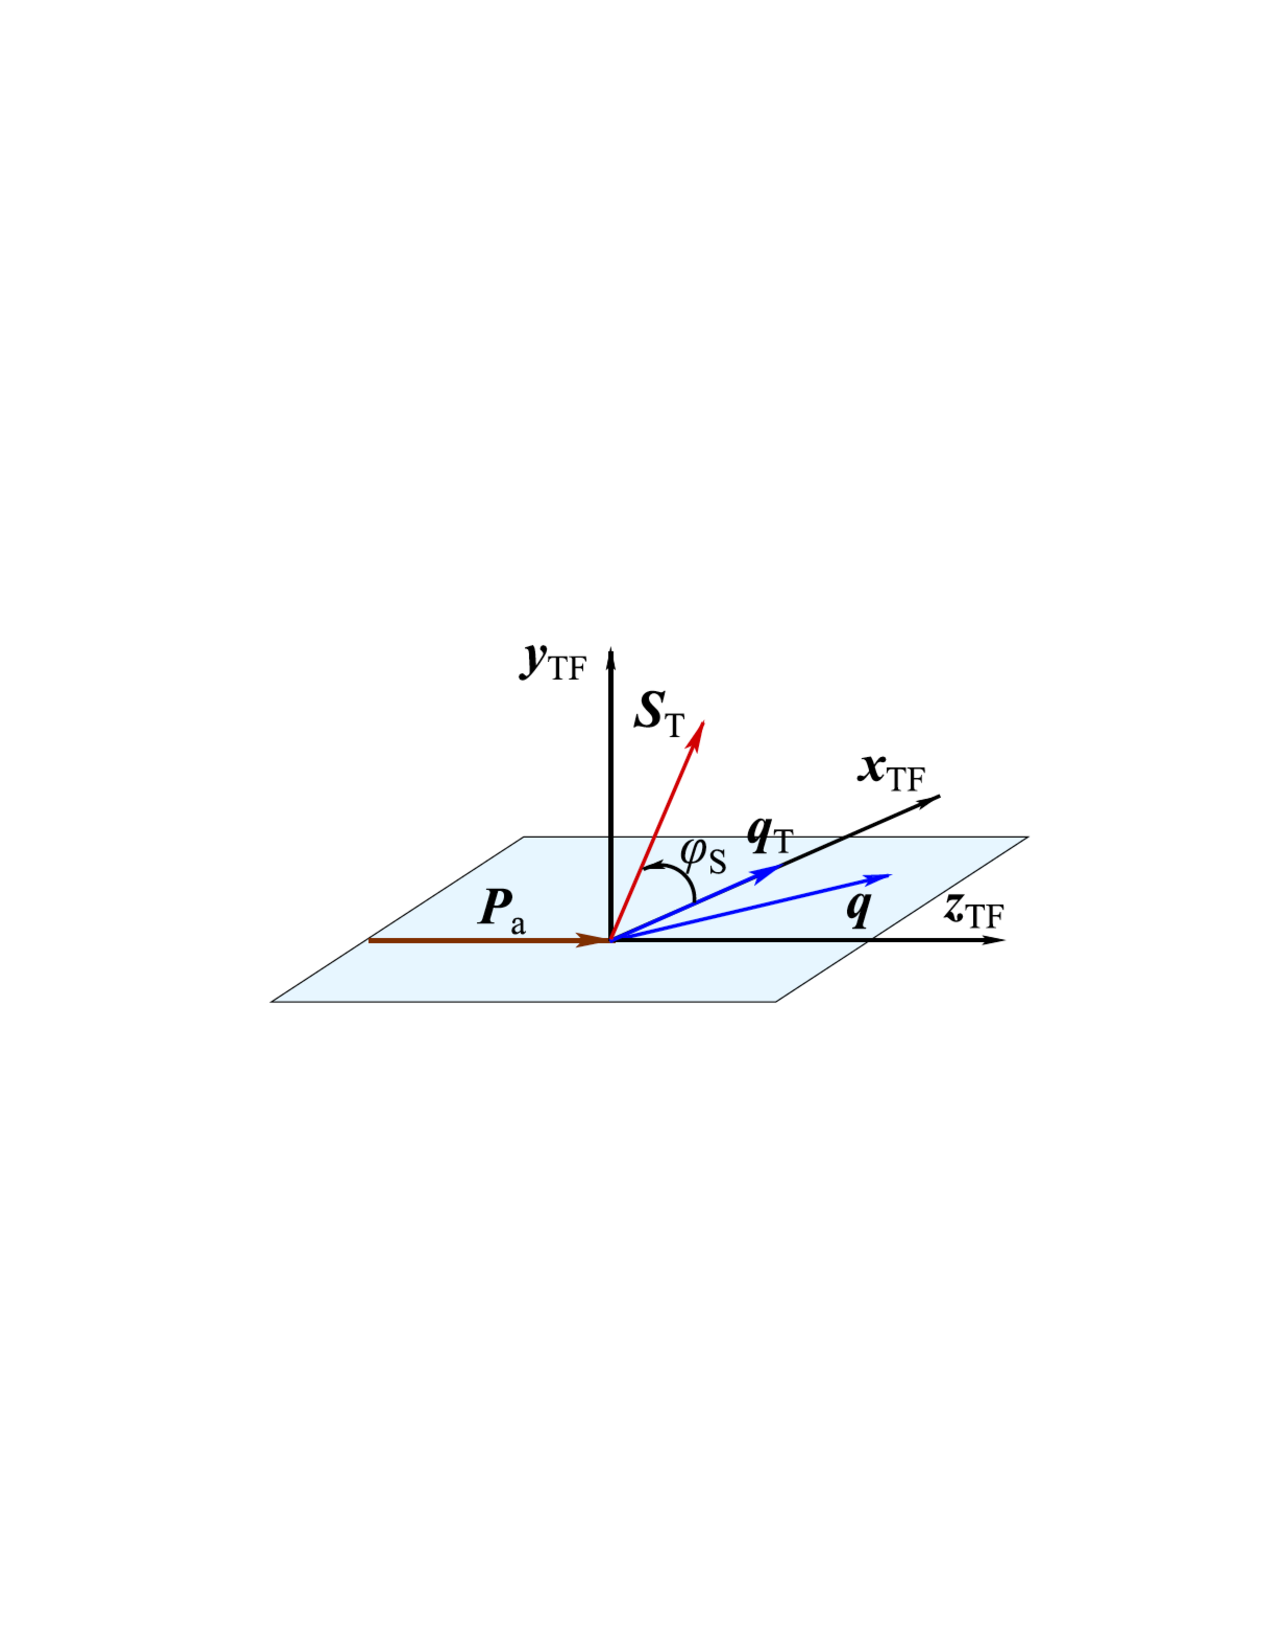
\includegraphics[width=\linewidth, trim=3cm 9cm 3cm 8cm,
      clip]{DY_TargetFrame}
    \caption{The target frame where the z-axis is along the beam and the x-axis
      is in the direction of the transverse momentum of the virtual photon.}
    \label{fig::DY_TargetFrame}%
  \end{subfigure}
  \begin{subfigure}{.02\textwidth}
    \centering
    
\includegraphics[width=\linewidth]{tmp}
    \label{fig::tmp1}%
  \end{subfigure}
  \begin{subfigure}{.46\textwidth}
    \centering
    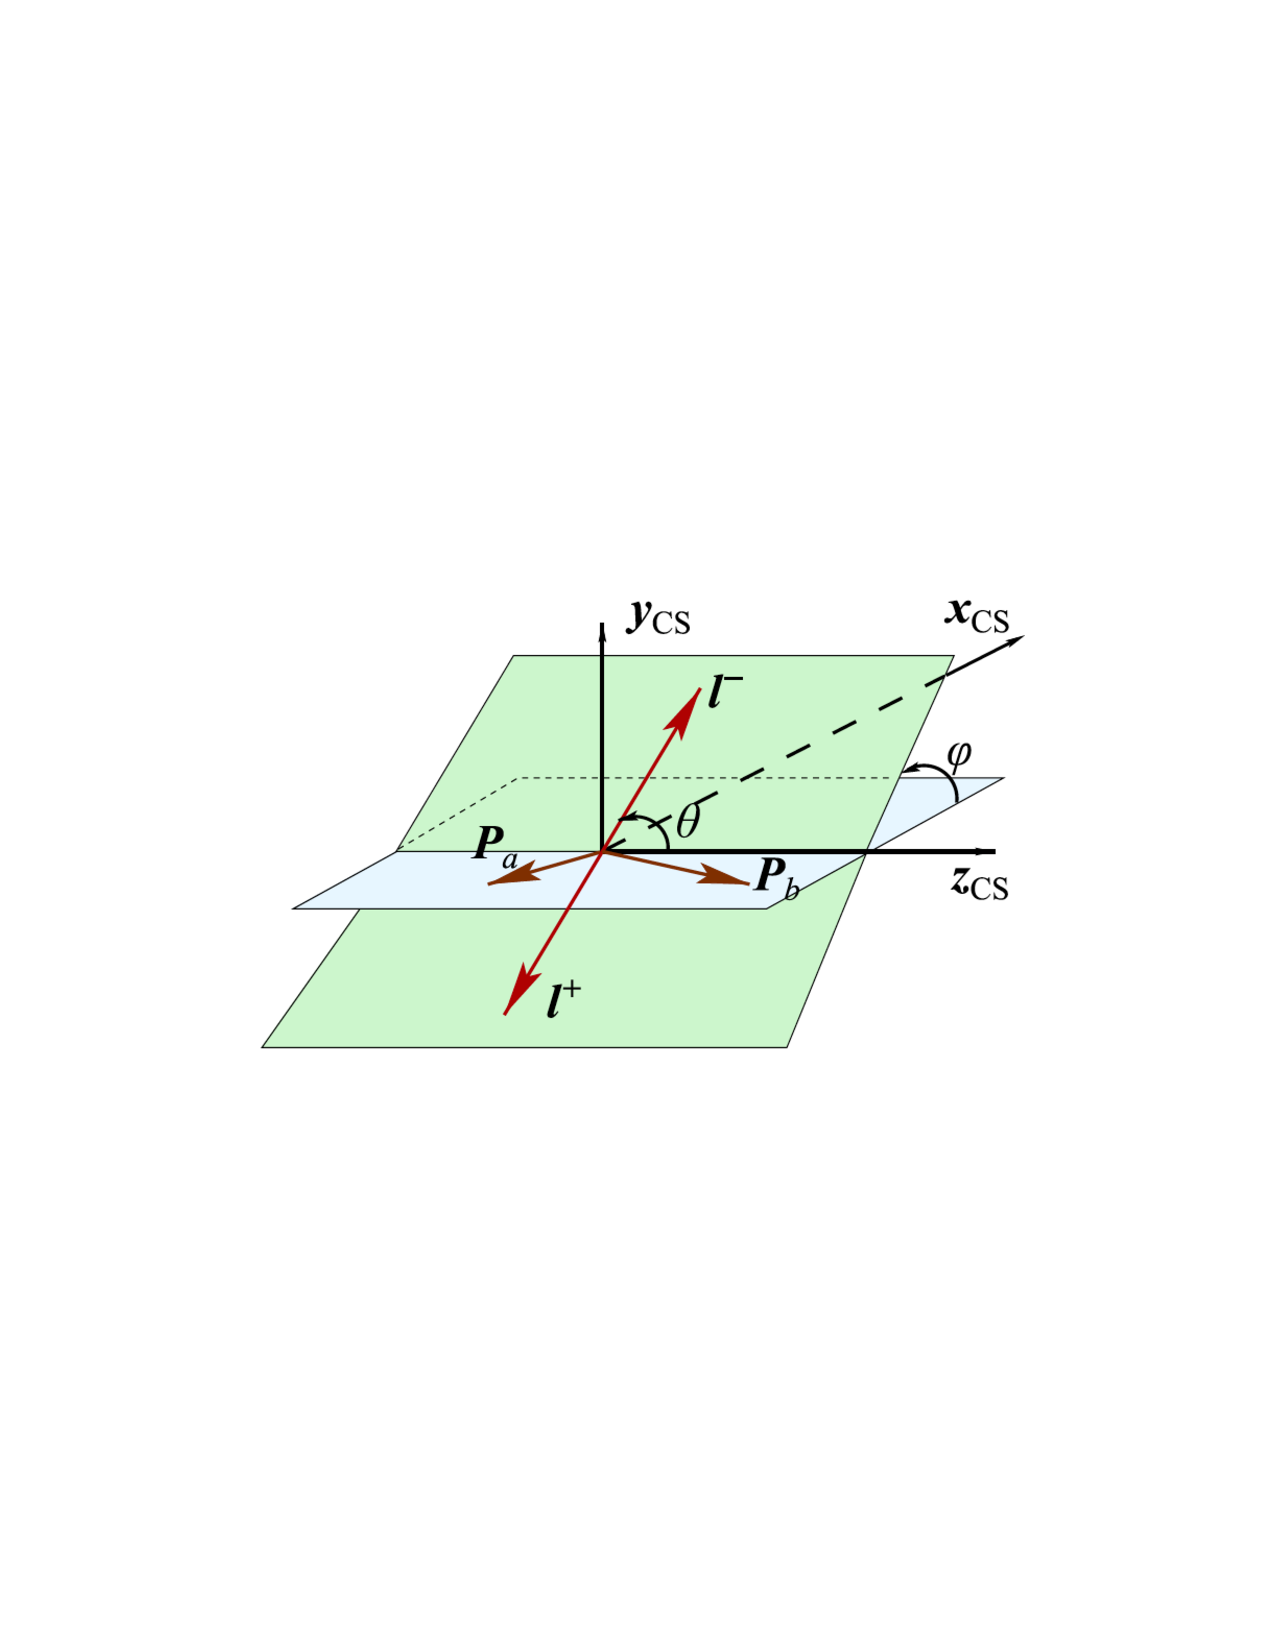
\includegraphics[width=\linewidth, trim=3cm 9cm 3cm 8cm,
      clip]{DY_CSFrame}
    \caption{The Collins-Soper frame is defined in the rest frame of the virtual
      photon where the z-axis bisects the beam and target momentum vectors.}
    \label{fig::DY_CSFrame}%
  \end{subfigure}
\end{figure}

The target frame is defined in the lab frame where the beam is along the z-axis
and the transverse momentum of the virtual photon is along the x-axis.  The
y-axis in the target frame is then chosen so the coordinate system is right
handed.  The Collins-Soper frame is defined in the rest frame of the virtual
photon where the xz-plane coincides with the hadron plane and the z-axis is
chosen so it bisects the momentum vectors $P_a$ and $-P_b$.  The CS frame is
defined from the target frame as a boost first along the along z-axis and then a
boost along the x-axis so the rest frame of the virtual photon is reached.

The leading order model independent Drell-Yan differential cross-section for a
polarized target is~\cite{DYxSection,AKotzininaNote}

\begin{align} \label{equ::DY_ang_dist}
  \frac{d\sigma}{d^4 q \, d \Omega} &=
  \frac{\alpha_{em}^2}{F \, q^2}
  \Big \{ \Big(
   (1 + \cos^2 \theta) \, F_{U}^{1} 
 + (1 - \cos^2 \theta) \, F_{U}^{2} 
 + \sin 2\theta \cos \phi \, F_{U}^{\cos \phi} 
 + \sin^2 \theta \cos 2\phi \, F_{U}^{\cos 2\phi} \Big)
 \nonumber \\
 &+ S_{L} \Big( 
   \sin 2\theta \sin \phi \, F_{L}^{\sin \phi} 
   + \sin^2 \theta \sin 2\phi \, F_{L}^{\sin 2\phi} \Big)
   \nonumber \\
   &+ |S_{T}|
   \Big[ \Big(
     F_{T}^{\sin \phi_S} + \cos^2 \theta \, \tilde{F}_{T}^{\sin \phi_S}
     \Big)\sin \phi_{S} 
     + \Big( F_{T}^{\sin (\phi +\phi_S)} \, \sin(\phi+\phi_S) +
     F_{T}^{(\sin \phi - \phi_S)}\, \sin(\phi-\phi_S) \Big)\sin 2\theta
     \nonumber \\
     & \quad\quad\quad +
     \Big( F_{T}^{\sin (2\phi +\phi_S)}\, \sin(2\phi+\phi_S) +
     F_{T}^{\sin (2\phi - \phi_S)}\, \sin(2\phi-\phi_S) \Big)\sin ^2\theta
     \Big ]
   \Big \},
\end{align}
\noindent
where $F = 4\sqrt{(P_a \cdot P_b)^2 - M_a^2M_b^2}$ is the flux and $\Omega$ is
the solid angle of the outgoing negatively charged muon.  The twelve model
independent structure functions in Eq.~\ref{equ::DY_ang_dist} are labeled as
$F_{Target \; polarization}^{azimuthal \;angle\;coefficient}$.  The phase space
when the TMD regime is valid in DY scattering is when $q_T << q$.  In this
regime the structure functions are equal to a convolution of a beam and a target
TMD function where convolution is defined similarly to the SIDIS case,
Eq.~\ref{equ::SIDIS_conv}, as

\begin{align}
  \label{equ::DY_conv}
  \nonumber
      {\cal C}\bigl[ w(k_{aT}, k_{bT}) f_a \bar{f}_b \bigr] =
      \frac{1}{N_c} \sum_q e_q^2 \int &d^2 k_{aT} d^2 k_{bT} 
      \delta^{(2)}\bigl(q_T - k_{aT} - k_{bT} \bigr) \\
      &\times w(k_{aT},k_{bT})
        \Big[ f_a^q(x,k_{aT}^2)f_b^{\bar{q}}(x,k_{bT}^2) +
          f_a^{\bar{q}}(x,k_{aT}^2)f_b^{q}(x,k_{bT}^2) \Big],
\end{align}
\noindent
where $N_c = 3$ is the number of color charges.  The leading order DY
structure functions in the TMD phase space are related to TMD functions
as~\cite{DYxSection}

\begin{align}
  \label{equ::DY_fU1}
  F_{U}^{1} &  =  
  {\cal C}  \big[ f_{1}  \bar{f}_{1} \big]
  &\propto f^{\bar{u}}_{1,Beam} \otimes f^u_{1,Target}, \\
  \label{equ::DY_fUcos2phi}
  F_{U}^{\cos 2\phi} &  =  
  {\cal C}  \Bigg[ \frac{2\big( \vec{h} \cdot \vec{k}_{aT} \big) 
                          \big( \vec{h} \cdot \vec{k}_{bT} \big)
                         - \vec{k}_{aT} \cdot \vec{k}_{bT}} {M_{a} M_{b}}  
    h_{1}^{\perp}  \bar{h}_{1}^{\perp} \Bigg]
  &\propto h^{\perp \, \bar{u}}_{1,Beam} \otimes h^{\perp \, u}_{1,Target}, \\
F_{L}^{\sin 2\phi} &  =  
-  {\cal C}  \Bigg[ \frac{2\big( \vec{h} \cdot \vec{k}_{aT} \big) 
                          \big( \vec{h} \cdot \vec{k}_{bT} \big)
                         - \vec{k}_{aT} \cdot \vec{k}_{bT}} {M_{a} M_{b}}  
                  h_{1}^{\perp}  \bar{h}_{1L}^{\perp} \Bigg]
&\propto h^{\perp \, \bar{u}}_{1,Beam} \otimes h^{\perp \, u}_{1L,Target}, \\
F_{T}^{1} &  =   
- {\cal C}  \Bigg[ \frac{\vec{h} \cdot \vec{k}_{bT}} {M_{b}}  
  f_{1}  \bar{f}_{1T}^{\perp} \Bigg]
&\propto f^{\bar{u}}_{1,Beam} \otimes f^{\perp \, u}_{1T,Target}, \\
F_{T}^{\sin (2\phi - \phi_S)} &  =  
-  {\cal C}  \Bigg[ \frac{\vec{h} \cdot \vec{k}_{aT}} {M_{a}} 
  h_{1}^{\perp}  \bar{h}_{1} \Bigg]
&\propto h^{\perp \, \bar{u}}_{1,Beam} \otimes h^{u}_{1,Target}, \\
\label{equ::DY_fTsin2phiphiS}
F_{T}^{\sin (2\phi + \phi_S)} &  =  
-  {\cal C}  \Bigg[ \frac{2\big( \vec{h} \cdot \vec{k}_{bT} \big)
                    \big[2 \big( \vec{h} \cdot\vec{k}_{aT} \big)
                         \big( \vec{h} \cdot \vec{k}_{bT} \big)
                        -\vec{k}_{aT} \cdot \vec{k}_{bT} \big]
                   - \vec{k}_{bT}^{2} \big( \vec{h} \cdot \vec{k}_{aT} \big)}
                  {2 M_{a} M_{b}^{2}}  
                  h_{1}^{\perp}  \bar{h}_{1T}^{\perp} \Bigg]
&\propto h^{\perp \, \bar{u}}_{1,Beam} \otimes h^{\perp \, u}_{1T,Target},
\end{align}

\noindent
where $\vec{h} = \vec{q}_T/q_T$ is a unit vector and furthermore the assumption
in this thesis is that the beam $\bar{u}$-quark annihilates with the target
u-quark.  The additional leading order structure functions are zero

\begin{equation}
  F_{U}^{2} \quad = \quad F_{U}^{\cos\phi} \quad = \quad F_{L}^{\sin\phi} \quad
  = \quad F_{T}^{2} \quad = \quad F_{T}^{\sin(\phi - \phi_S)} \quad = \quad
  F_{T}^{\sin(\phi + \phi_S)} \quad = 0.
\end{equation}

The differential cross-seciton, Eq.~\ref{equ::DY_ang_dist}, can be rewritten in
terms of asymmetry amplitudes and depolarization factors.  The asymmetry
amplitudes are defined similarly to the case in SIDIS,
Eq.~\ref{equ::asymAmpSIDIS}, and again for the reason that asymmetries can be
determined to a higher precision than structure functions.  For Drell-Yan these
asymmetry amplitudes are

\begin{equation}
  A^{w_i(\phi, \phi_S)}_{Target} = \frac{F^{w_i(\phi,
      \phi_S)}_{Target}}{F_{U}^1+F_{U}^2}.
  \label{equ::asymAmpDY}
\end{equation}
\noindent
The asymmetry amplitudes are the result of different virtual photon
polarizations decaying to a final state lepton pair.  The depolarization factor
is defined as the ratio of the virtual photon polarization to produce such an
asymmetry to that of a transversely polarized virtual photon.  The
depolarization is defined for each asymmetry amplitude as

\begin{equation}
  D_{[f(\theta)]} = \frac{f(\theta)}{1+A_U^1\;\cos^2\theta},
\end{equation}
\noindent
where the function $f(\theta)$ corresponds to virtual photon angular decay
responsible for the given asymmetry.  The Drell-Yan differential cross-section,
Eq.~\ref{equ::DY_ang_dist}, now simplifies to~\cite{AKotzininaNote}

\begin{align}
  \label{equ::DY_usefulXsect}
  \frac{d\sigma}{d^4 q \, d \Omega} &=
  \frac{\alpha_{em}^2}{F \, q^2}\hat{\sigma}_U
  \Big \{ \Big(1 + D_{[\sin^2 \theta]} \cos 2\phi \, A_{U}^{\cos 2\phi} \Big)
 \nonumber \\
 &+ S_{L} D_{[\sin^2 \theta]} \sin 2\phi \, A_{L}^{\sin 2\phi}
   \nonumber \\
   &+ |S_{T}|
   \Big[A_{T}^{\sin \phi_S}\;\sin \phi_{S} 
     + \Big( A_{T}^{\sin (2\phi +\phi_S)}\, \sin(2\phi+\phi_S) +
     A_{T}^{\sin (2\phi - \phi_S)}\, \sin(2\phi-\phi_S) \Big)D_{[\sin ^2\theta]}
     \Big ]
   \Big \},
\end{align}
\noindent
where $\hat{\sigma}_U = F^1_U (1+\cos^2\theta)$ is the unpolarized DY
cross-section.  For the data taking conditions in 2015 it is assumed that the target is transversely polarized so $S_L = 0$ and therefore the Drell-Yan cross-section can be simplified to

\begin{align}
  \label{equ::DY_MostusefulXsect}
  \frac{d\sigma}{d^4 q \, d \Omega} &=
  \frac{\alpha_{em}^2}{F \, q^2}\hat{\sigma}_U
  \Big \{ \Big(1 + D_{[\sin^2 \theta]} \cos 2\phi \, A_{U}^{\cos 2\phi} \Big)
   \nonumber \\
   &+ |S_{T}|
   \Big[A_{T}^{\sin \phi_S}\;\sin \phi_{S} 
     + \Big( A_{T}^{\sin (2\phi +\phi_S)}\, \sin(2\phi+\phi_S) +
     A_{T}^{\sin (2\phi - \phi_S)}\, \sin(2\phi-\phi_S) \Big)D_{[\sin ^2\theta]}
     \Big ]
   \Big \}.
\end{align}

\subsection{Drell-Yan Sivers Result}
The first Drell-Yan results for the Sivers asymmetry amplitude, in an attempt to
verify the sign change between Drell-Yan and SIDIS, came from hadron-hadron
collisions at Star~\cite{PhysRevLett.116.132301}.  Their result measured the
Sivers amplitude from $pp^{\uparrow} \rightarrow Z^0X$ and $pp^{\uparrow}
\rightarrow W^{\pm}X$ and are shown in Fig.~\ref{fig::StarSivers}.  The
statistical error bars are too high and the $Q^2$ scale is very different from
that used to measure a Sivers function in SIDIS however.  As of the data of this
thesis it is impossible to conclude on a sign change of the Sivers function
between Drell-Yan and SIDIS.

\begin{figure}[h!t]
  \centering
  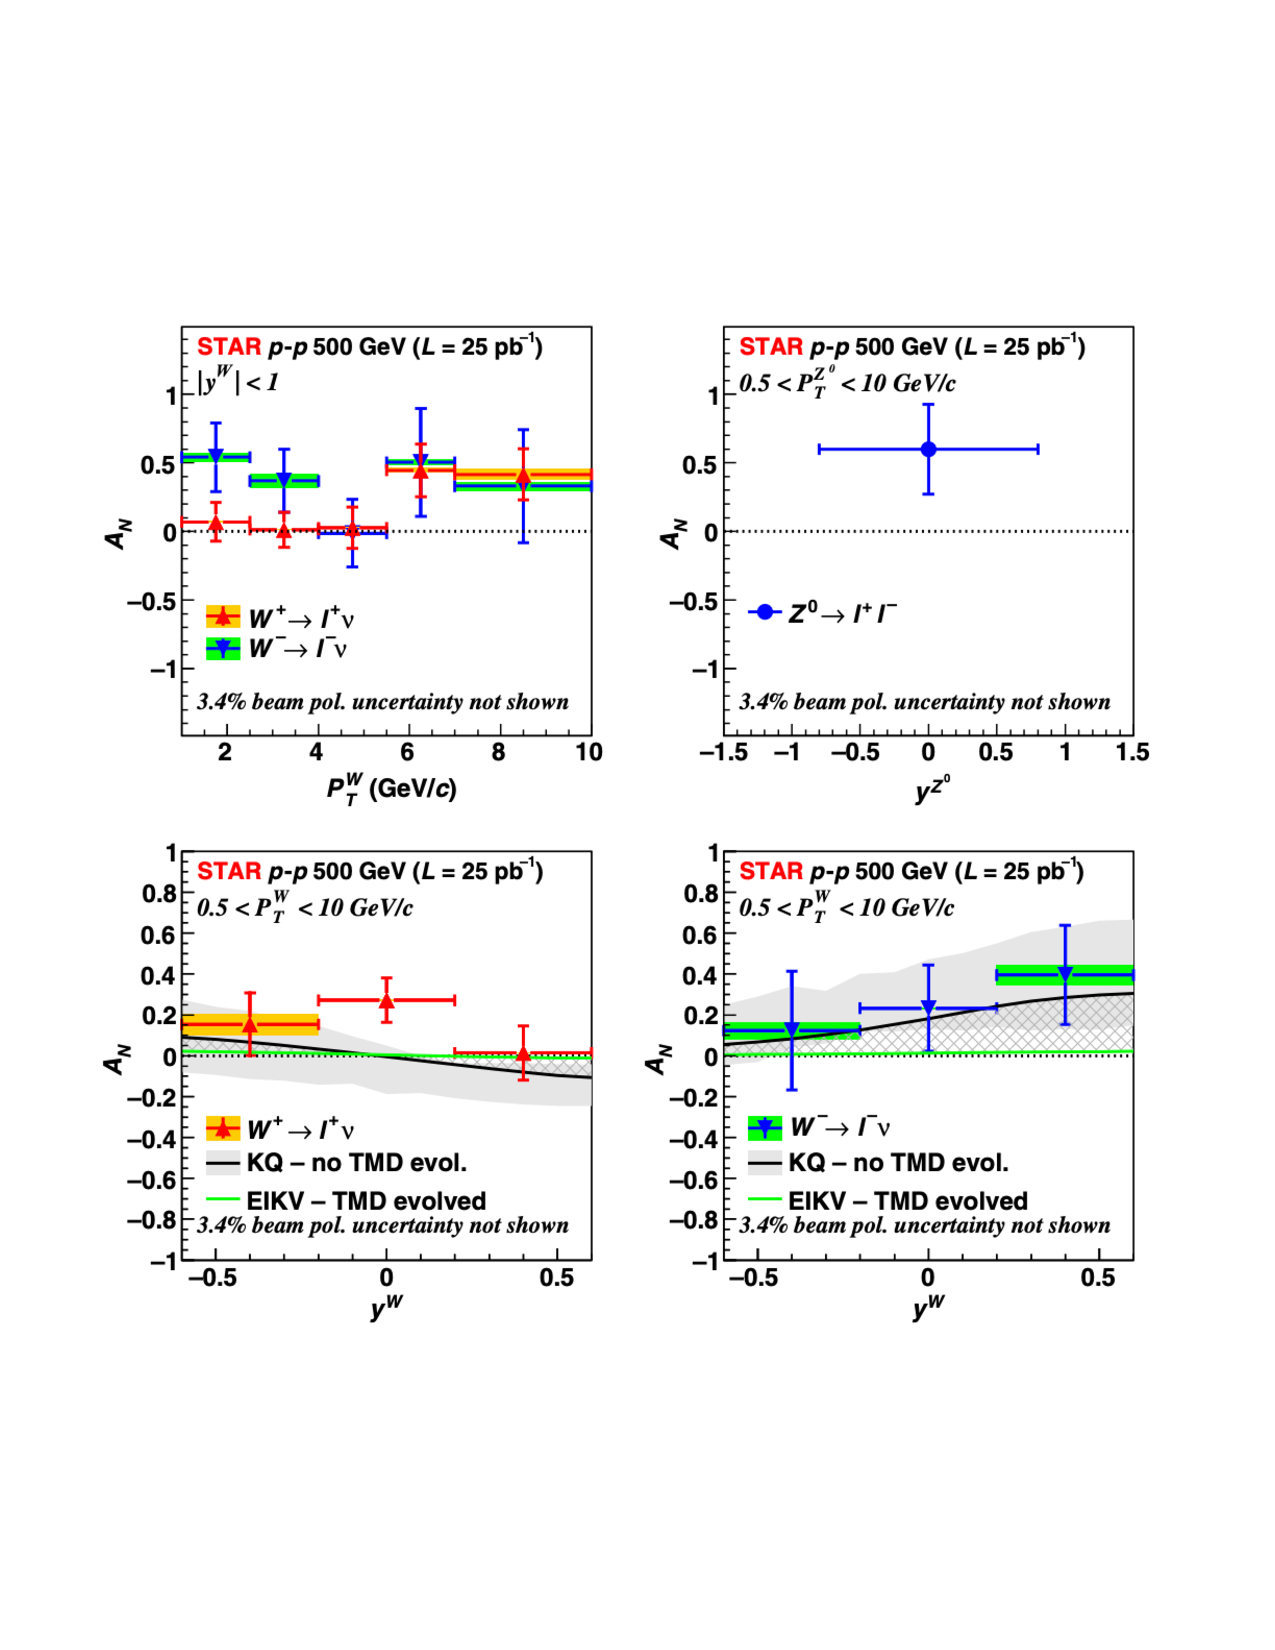
\includegraphics[width=0.7\textwidth, trim=1cm 5cm 1cm 5cm]{StarSivers}
  \caption{All plots show a left-right asymmetry which is related to the Sivers
    function.  The top right plot is for $Z^0$ production while the other three
    plots are for $W^\pm$ production.  $Q^2$ evolution and resulting error bars
    from EIKV~\cite{PhysRevD.89.074013} and KQ~\cite{PhysRevLett.103.172001}.
    Image taken from~\cite{PhysRevLett.116.132301}.}
  \label{fig::StarSivers}
\end{figure}

\subsection{Left-Right Asymmetry} \label{sec::lr_theory}
An asymmetry of interest for measuring high energy spin related phenomena is the
analyzing power.  This asymmetry is denoted $A_N$ and is responsible for a
left-right asymmetry for a suitable definition of left and right.  The
cross-section for spin 1/2 particles scattering where one of the initial
particles is polarized can be written

\begin{equation}
  \label{equ::AN_xsect}
  I(\theta, \phi) = I_0(\theta)(1+SA_N \cos(\phi))
\end{equation}
\noindent
where $I_0$ is the unpolarized cross-section, $S$ is the beam or target
polarization percentage and $\phi$ is the azimuthal scattering angle of the
outgoing measured particle.  Working in the target frame for Drell-Yan
scattering from a transversely polarized target, the azimuthal angle can be
redefined in terms of the $\phi_S$ angle by noting that $\phi = \frac{\pi}{2} -
\phi_S$. Eq.~\ref{equ::AN_xsect} can then be written in the form of the
Drell-Yan cross-section, Eq.~\ref{equ::DY_usefulXsect}, as

\begin{align}
  \frac{d\sigma}{d^4 q \, d \phi_S} &= \frac{\alpha_{em}^2}{F \,
    q^2}\hat{\sigma}_U\Big(1+|S_T|A_N \cos (\frac{\pi}{2} - \phi_S) \Big)
  \\ \nonumber
  &= \frac{\alpha_{em}^2}{F \,
    q^2}\hat{\sigma}_U\Big(1+|S_T|A_N \sin(\phi_S) \Big)
  \\ \nonumber
  &= \frac{\alpha_{em}^2}{F \,
    q^2}\hat{\sigma}_U \Big(1+|S_T| A_{T}^{\sin \phi_S} \sin(\phi_S)\Big),
\end{align}
\noindent
where this relation is obtained from Eq.~\ref{equ::DY_usefulXsect} by
integrating over all angle except $\phi_S$ and where the polarization $S$ is
assumed to be transverse.  Therefore the analyzing power, $A_N$, is the same as
the Sivers asymmetry amplitude, $A_{T}^{\sin \phi_S}$, for Drell-Yan scattering.

An analysis technique for measuring $A_N$ is by making a left-right asymmetry.
The left-right asymmetry is defined as 
\begin{equation}
  A_{lr} = \frac{1}{P}\frac{\sigma_{left} -
    \sigma_{right}}{\sigma_{left} + \sigma_{right}},
\end{equation}
\noindent
where $\sigma_{left(right)}$ is the cross-section for producing a final state to
the left(right).  In the target frame the definition of left scattering is
$\int_{\phi_S=0}^{\phi_S=\pi}\frac{d\sigma}{d^4 q \, d \phi_S} d\phi_S$ and
definition of right scattering is
$\int_{\phi_S=\pi}^{\phi_S=2\pi}\frac{d\sigma}{d^4 q \, d \phi_S} d\phi_S$.  It
is straight forward to show the relationship between $A_{lr}$ and $A_N$ as

\begin{align}
  A_{lr} &= \frac{1}{|S_T|}
  \frac{\int_{\phi_S=0}^{\phi_S=\pi} \frac{d\sigma}{d^4 q \, d \phi_S}d\phi_S
    - \int_{\phi_S=\pi}^{\phi_S=2\pi}\frac{d\sigma}{d^4 q \, d \phi_S}d\phi_S}
       {\int_{\phi_S=0}^{\phi_S=\pi}\frac{d\sigma}{d^4 q \, d \phi_S}d\phi_S
         + \int_{\phi_S=\pi}^{\phi_S=2\pi}\frac{d\sigma}{d^4 q \, d \phi_S}d\phi_S}
       \\ \nonumber
       &= \frac{1}{|S_T|}
       \frac{\phi_S -|S_T|A_N\cos\phi_S \Big|_0^{\pi}
       - \Big(\phi_S -|S_T|A_N\cos\phi_S \Big|_{\pi}^{2\pi}\Big)}
            {\phi_S -|S_T|A_N\cos\phi_S \Big|_0^{\pi}
              + \Big(\phi_S -|S_T|A_N\cos\phi_S \Big|_{\pi}^{2\pi}\Big)}
            \\ \nonumber
            &= \frac{1}{|S_T|}
            \frac{4|S_T|A_N}{2\pi}
            \\ \nonumber
            &= \frac{2A_N}{\pi}.
\end{align}

Another method to determine $A_N$, is with the transverse spin asymmetry (TSA)
defined as
\begin{align}
  \label{equ::AN_TSA}
  A_{TSA} =& \frac{1}{|S_T|} \frac{\frac{d\sigma^{\uparrow}}{d\phi_s} -
    \frac{d\sigma^{\downarrow}}{d\phi_s}} {\frac{d\sigma^{\uparrow}}{d\phi_s} +
    \frac{d\sigma^{\downarrow}}{d\phi_s}} \\ \nonumber =& \frac{1}{|S_T|} \frac{1 +
    |S_T|A_N\sin\phi_S - \Big(1 + |S_T|A_N\sin(\phi_S + \pi) \Big)} {1 + |S_T|A_N\sin\phi_S
    + \Big(1 + |S_T|A_N\sin(\phi_S + \pi) \Big)} \\ \nonumber =& A_N\sin\phi_S.
\end{align}

To understand how $A_N$ is related to the Sivers function, it is illustrative to
write the Drell-Yan differential cross-section under the TMD assumptions
as~\cite{PhysRevLett.103.172001}
\begin{equation}
  \frac{d\sigma^{H_aH_b\rightarrow l^+l^- X}}{d\eta dM^2d^2q_T} =
  \hat{\sigma}_0 \sum_q e^2_q \int d^2k_{aT} d^2k_{bT}
  \delta^{(2)}(k_{aT}+k_{bT}-q_T)
  f_{\bar{q}/H_a}(x_a, k_{aT})f_{q/H_b}(x_b, k_{bT}),
\end{equation}
\noindent
 $\eta$ is rapidity and $f_{\bar{q}(q)/H_{a(b)}}$ is a TMD function.  Inserting
this cross-section into the transverse spin asymmetry, Eq.~\ref{equ::AN_TSA},
and using proper TMD functions for the given transverse polarization gives
\begin{align}
  A_{TSA} &= A_N \sin \phi_S
  \\ \nonumber
  &= -\frac{1}{S}
  \frac{\sum_q e^2_q \int d^2k_{aT} d^2k_{bT}
    \delta^{(2)}(k_{aT}+k_{bT}-q_T)f_{\bar{q}/H_a}(x_a, k_{aT})
    \frac{k_{bT}}{M_b}f_{1T}^{\perp q}(x_b, k_{bT})
    S\sin \phi_S}
  {\sum_q e^2_q \int d^2k_{aT} d^2k_{bT}
    \delta^{(2)}(k_{aT}+k_{bT}-q_T)
    f_{\bar{q}/H_a}(x_a, k_{aT})f_{q/H_b}(x_b, k_{bT})}.
\end{align}

Several experiments measured large values for $A_N$ at different center of mass
energies.  Fig.~\ref{fig::AN_vsXF} shows the results of $A_N$ from hadron-hadron
collisions from four different experiments over a range of center of mass
energies.

\begin{figure}[h!t]
  \centering
  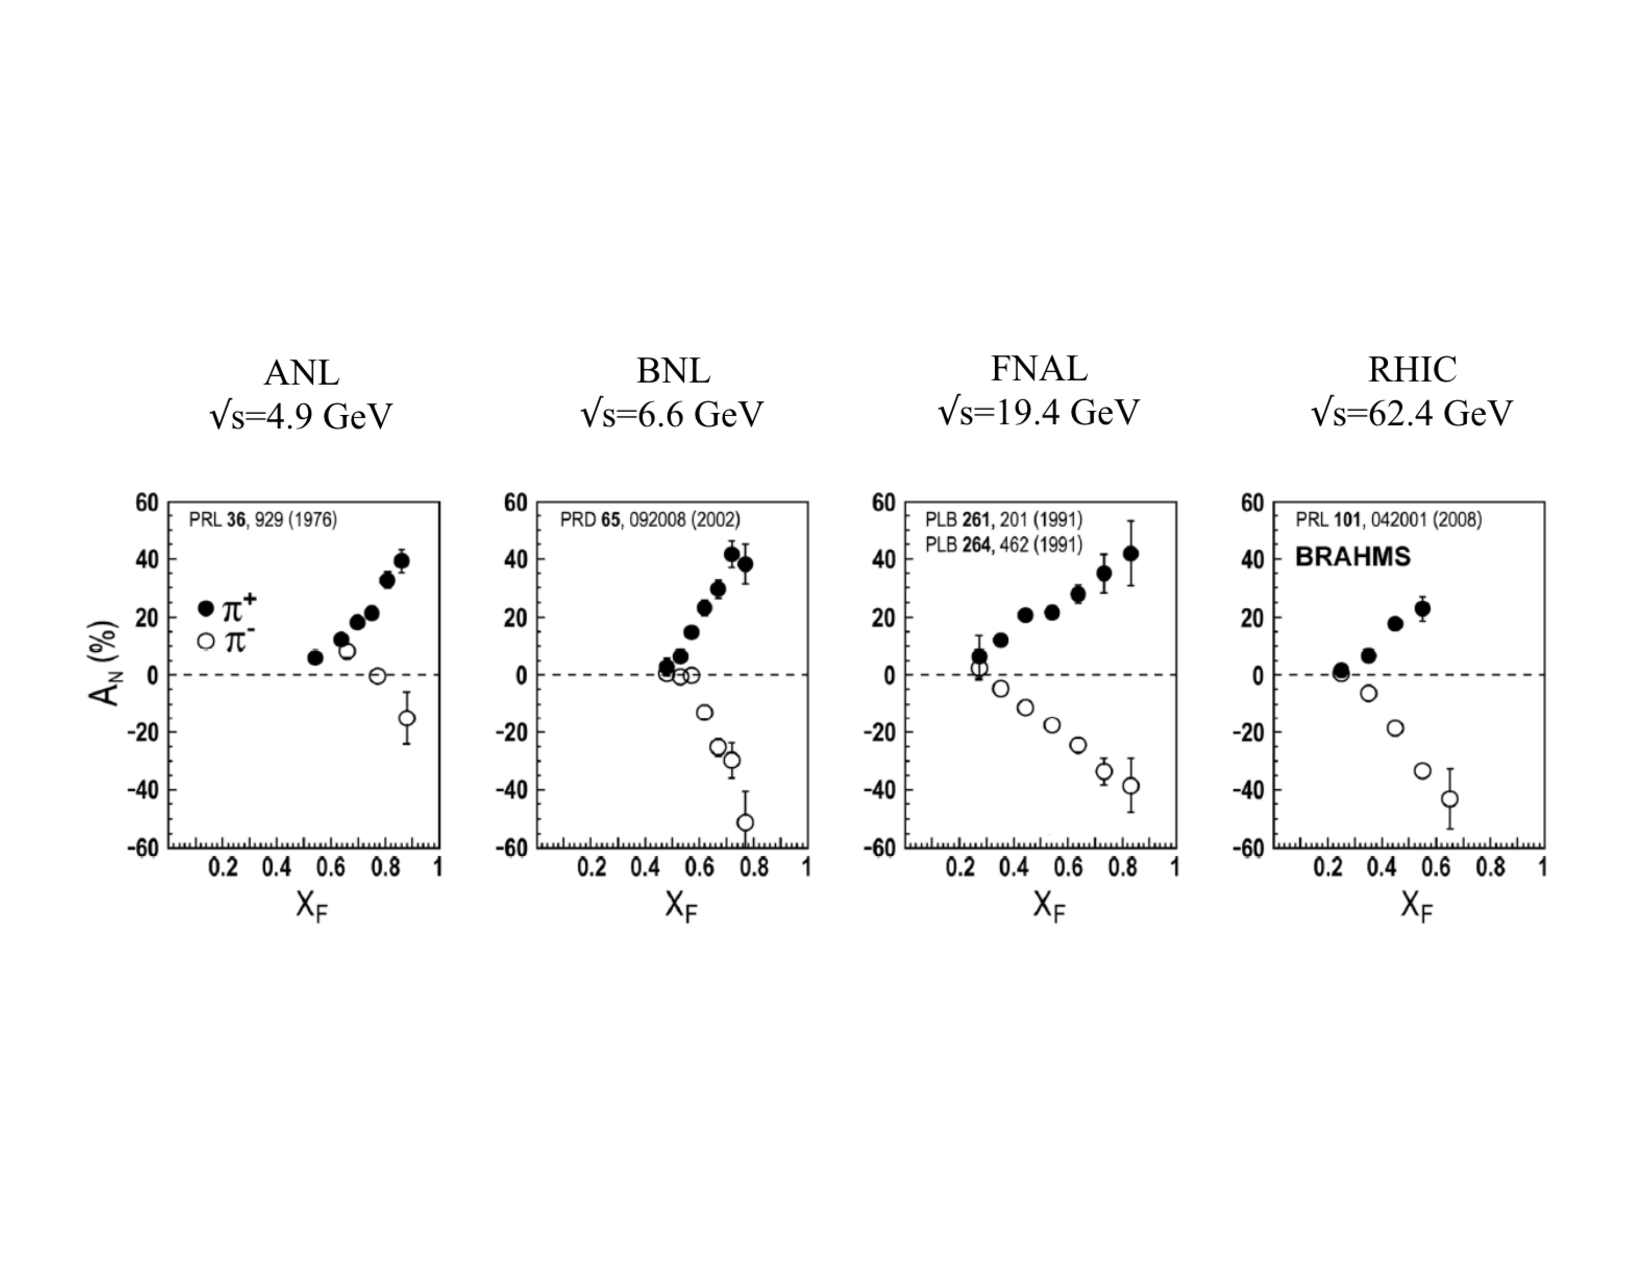
\includegraphics[width=0.9\textwidth, trim=1cm 6cm 1cm 6cm, clip]{AN_vsXF}
  \caption{Large $A_N$ values where found at ANL~\cite{PhysRevLett.36.929},
    BNL~\cite{PhysRevD.65.092008}, FNAL~\cite{ADAMS1991201,ADAMS1991462} and
    RHIC~\cite{PhysRevLett.101.042001}.}
  \label{fig::AN_vsXF}
\end{figure}

\subsection{Weighted Asymmetries from Drell-Yan}\label{sec::qt_w_theory}

The proton TMD functions, determined from Drell-Yan in
Eqs.~\ref{equ::DY_fU1}-\ref{equ::DY_fTsin2phiphiS}, are convoluted with a TMD
function from the beam pion.  The Drell-Yan convolution, Eq.~\ref{equ::DY_conv},
makes it difficult to determine a single TMD function and for this reason model
assumptions are made in the global analysis to extract the individual TMDs from
the convolutions.  An alternative method involving weighted asymmetries however,
makes it possible to disentangle the convolution and determine a $k_T^2$ moment
of a TMD function both for
SIDIS~\cite{Kotzinian:1995cz,Kotzinian:1997wt,Boer:1997nt} and for
Drell-Yan~\cite{Efremov:2004tp,Sissakian:2005vd,Sissakian:2005yp,Wang:2017onm}.

The deconvolution by weighted asymmetries works by multiplying a given structure
function by an appropriate weight and integrating over the virtual photon
transverse momentum, $q_T$.  The simplest Drell-Yan structure function to
deconvolute is $F_U^1$.  By integrating Eq.~\ref{equ::DY_fU1} over $q_T$ the
convolution equation becomes

\begin{align}
  \label{equ::DY_fu1_qtint}
  \int d^2{q_T} F_U^1 &=
  \int d^2{q_T} {\cal C}  \big[ f_{1,a} \bar{f}_{1,b} \big]
  \\ \nonumber
  &= \int d^2{q_T} \frac{1}{N_c} \sum_q e_q^2 \int d^2 k_{aT} d^2 k_{bT} 
  \delta^{(2)}\bigl(q_T - k_{aT} - k_{bT} \bigr)
  \\ \nonumber
  & \quad\quad\quad
  \times \Big[ f_{1,a}^q(x_a,k_{aT}^2)f_{1,b}^{\bar{q}}(x_b,k_{bT}^2) +
    f_{1,a}^{\bar{q}}(x_a,k_{aT}^2)f_{1,b}^{q}(x_b,k_{bT}^2) \Big]
  \\ \nonumber
  &= \frac{1}{N_c} \sum_q
  e_q^2 f_{1,a}^q(x_a)f_{1,b}^{\bar{q}}(x_b) +
  f_{1,a}^{\bar{q}}(x_a)f_{1,b}^{q}(x_b)
  \\ \nonumber
   \substack{COMPASS \\ \approx} \quad &
   \frac{4}{27}f_{1,\pi}^{\bar{u}}(x_\pi)f_{1,proton}^u(x_{proton}),
\end{align}

\noindent
where $f_1(x) = \int d^2 k_{T} f_1(x,k_{T}^2)$ is a TMD function integrated over
$k_T$.  In Eq.~\ref{equ::DY_fu1_qtint} the weight was 1 and no assumptions were
needed to perform the integration.  The answer is a TMD function for the beam
multiplied by a TMD function from the target.  The final equality in
Eq.~\ref{equ::DY_fu1_qtint} is valid in the COMPASS kinematic region and shows
how straight forward this method can make TMD extraction.

Deconvoluting the additional Drell-Yan structure functions,
Eqs~\ref{equ::DY_fUcos2phi}-\ref{equ::DY_fTsin2phiphiS}, is similar to
Eq.~\ref{equ::DY_fu1_qtint} but requires a different weight.  The Sivers TMD
function can be extracted from the $F_T^1$ structure function using a weight
equal to $|q_T|/M_b$.  This can be seen by multiplying $F_T^1$ by the weight
$|q_T|/M_b$, and integrating over $q_T$ to remove the Dirac delta function as
follows

\begin{align}
  \label{equ::DY_ft_qtint}
  \int d^2{q_T} \frac{|q_T|}{M_b} F_T^1 &=
  - \int d^2{q_T} \frac{|q_T|}{M_b} {\cal C}
  \Big[\frac{\vec{q}_T \cdot \vec{k}_{bT}} {|q_T|M_{b}}  
  f_{1,a}  \bar{f}_{1T,b}^{\perp} \Big]
  \\ \nonumber
  &= - \int d^2{q_T} \frac{|q_T|}{M_b}
  \frac{1}{N_c} \sum_q e_q^2 \int d^2 k_{aT} d^2 k_{bT} 
  \delta^{(2)}\bigl(q_T - k_{aT} - k_{bT} \bigr)
  \\ \nonumber
  & \quad\quad\quad
  \times \frac{\vec{q}_T \cdot \vec{k}_{bT}} {|q_T|M_{b}}
  \Big[ f_{1,a}^q(x_a,k_{aT}^2)f_{1T,b}^{\bar{q}\perp}(x_b,k_{bT}^2) +
    f_{1,a}^{\bar{q}}(x_a,k_{aT}^2)f_{1T,b}^{q\perp}(x_b,k_{bT}^2) \Big]
  \\ \nonumber
  &= - \frac{1}{N_c} \sum_q e_q^2 \int d^2 k_{aT} d^2 k_{bT} 
  \times \frac{(\vec{k}_{aT} + \vec{k}_{bT}) \cdot \vec{k}_{bT}} {M^2_{b}}
  \Big[ f_{1,a}^q(x_a,k_{aT}^2)f_{1T,b}^{\bar{q}\perp}(x_b,k_{bT}^2) +
    f_{1,a}^{\bar{q}}(x_a,k_{aT}^2)f_{1T,b}^{q\perp}(x_b,k_{bT}^2) \Big].
\end{align}
\noindent
To simplify further we make use of the fact that the unpolarized quark
distribution function is even in $k_T$ which means
\begin{equation}
  \int_{-\infty}^{\infty} d^2 k_{aT} \vec{k}_{aT} \cdot \vec{k}_{bT}
  f_{1,a}(x_a, k_{aT}^2) = 0,
\end{equation}
\noindent
and therefore only even terms in $k_T^2$ need to be
considered. Eq.~\ref{equ::DY_ft_qtint} can then be further simplified as

\begin{align}
  \int d^2{q_T} \frac{|q_T|}{M_b} F_T^1 &=
  - \frac{2}{N_c} \sum_q e_q^2
  \Big[ f_{1,a}^q(x_a) f_{1T,b}^{(1)\bar{q}\perp}(x_b) +
    f_{1,a}^{\bar{q}}(x_a) f_{1T,b}^{(1)q\perp}(x_b) \Big]
  \\ \nonumber
  \substack{COMPASS \\ \approx}& \quad
  - \frac{8}{27}
  f_{1,\pi}^{\bar{u}}(x_\pi)f_{1T,proton}^{(1)u\perp}(x_{proton}),
\end{align}
\noindent
where the $f_{1T}^{(1)q\perp}(x) = \int d^2 k_{T}
\frac{k_T^2}{2M}f_{1T}^{q\perp}(x, k_T^2)$ is the first $k_T^2$ moment of the
Sivers function and the general $k_T$ moment of a TMD is defined as $f^{(n)}(x)
= \int d^2 k_{T} \Big(\frac{k_T^2}{2M}\Big)^nf(x, k_T^2)$.

The essential steps in deconvolution the TMD functions are to multiply by a
weight which gets rid of any ${q_T}$ terms outside of the Dirac delta function
and to only include even terms in $k_T$.  The remaining two transverse
spin-dependent structure functions can also be deconvoluted in a similar fashion
to give

\begin{align}
  \label{equ::DY_fpretz_qtint}
  \int d^2{q_T} \frac{|q_T|^3}{2M_aM_b^2} F_T^{\sin(2\phi+\phi_S)} &=
  - \frac{2}{N_c} \sum_q e_q^2 \Big[
    h_{1,a}^{(1)\bar{q}\perp}(x_a)h_{1T,b}^{(2)q\perp}(x_b) +
    (q\leftrightarrow\bar{q})
    \Big]
  \\ \nonumber
  \substack{COMPASS \\ \approx} & \;
  - \frac{8}{27} h_{1,\pi}^{(1)\bar{u}\perp}(x_{\pi})\;
  h_{1T,proton}^{(2)u\perp}(x_{proton}),
  \\ \nonumber
  \\
  \label{equ::DY_ftrans_qtint}
  \int d^2{q_T} \frac{|q_T|}{M_a} F_T^{\sin(2\phi-\phi_S)} &=
  - \frac{2}{N_c} \sum_q e_q^2 \Big[
    h_{1,a}^{(1)\bar{q}\perp}(x_a)h_{1,b}^{(2)q}(x_b) +
    (q\leftrightarrow\bar{q})
    \Big]
  \\ \nonumber
  \substack{COMPASS \\ \approx} & \;
  - \frac{8}{27} h_{1,\pi}^{(1)\bar{u}\perp}(x_{\pi})\;
  h_{1,proton}^{(2)u}(x_{proton}),
\end{align}
\noindent
where Eq.~\ref{equ::DY_fpretz_qtint} can be used to determined the proton
pretzelosity function and Eq.~\ref{equ::DY_ftrans_qtint} can be used to
determine the proton transversity function.

For experimentally determining the $k_T^2$ moments of TMD functions the
following weighted asymmetries amplitudes are defined

\begin{equation}
  A^{YW_Y}{X}(x_a, x_b) = \frac{\int d^2{q_T} W_YF^Y_X}{\int d^2{q_T} F_U^1},
\end{equation}
\noindent
where $Y$ is the azimuthal modulation of interest, $W_Y$ is the appropriate
weight and $X$ denotes the targets polarization.  For example the Sivers
weighted asymmetry amplitude is as follows

\begin{equation}
  A^{\sin \phi_S \frac{q_T}{M_b}} =
  \frac{\int d^2{q_T} \frac{q_T}{M_b}F^{\sin \phi_S}_T}{\int d^2{q_T} F_U^1}
  \quad\quad \substack{COMPASS \\ \approx} \;
  -2\frac{f_{1T,proton}^{(1)u\perp}(x_{proton})}{f_{1,proton}}.
\end{equation}

\subsection{J/$\Psi$ Production}
The production of J/$\Psi$ hadrons potentially offers an alternative mechanism
for studying TMD related effects.  As of yet however, there is no confirmation
on the J/$\Psi$ production mechanism and therefore it impossible to say if TMD
effects are present from J/$\Psi$ production.  Still there are many models which can
be tested, some of which assume TMD functions contribute to produce J/$\Psi$
hadrons.

One of the most popular J/$\Psi$ production models, is the color evaporation
model~\cite{VOGT1999197}.  In this model the J/$\Psi$ production results from
gluon-gluon fusion and quark and ant-quark annihilation.  This is depicted as

\begin{equation}
  \sigma \Big |_{H_aH_b\rightarrow J/\Psi X \rightarrow l^+l^- X}
  = \sigma_{q\bar{q}\rightarrow c\bar{c}} + \sigma_{gg\rightarrow c\bar{c}},
\end{equation}

\noindent
where $\sigma_{q\bar{q}(gg)\rightarrow c\bar{c}}$ is the cross-section for
quark-quark annihilation (gluon-gluon fusion) to a $c\bar{c}$ final state.  In
the case of quark-quark annihilation there is interest in a model duality
between Drell-Yan and J/$\Psi$ production.

The spin and parity J/$\Psi$ quantum numbers are the same as the spin and parity
of a photon.  For this reason it is hypothesized that there is a duality between
the Drell-Yan process and J/$\Psi$
production~\cite{Anselmino:2004ki,Barone2007,Sissakian:2008th}.  This duality
transforms the electromagnetic coupling and Drell-Yan invariant mass to a new
J/$\Psi$ coupling and J/$\Psi$ mass given as

\begin{align}
  \nonumber
  \mathrm{Drell-}\mathrm{Yan}\; \mathrm{Production} \quad &
  \quad\quad\quad\quad \mathrm{J/}\Psi \;\mathrm{Production}
  \\
  \label{equ::dualityJPsi_coupling}
  16\pi^2\alpha^2e_q^2 \quad &\rightarrow
  \quad \quad\quad (g_q^{J/\Psi})^2(g_l^{J/\Psi})^2
  \\
  \label{equ::dualityJPsi_mass}
  \frac{1}{M^4} \quad \quad &\rightarrow \quad
  \frac{1}{(M^2-M^2_{J/\Psi})^2 + M^2_{J/\Psi}\Gamma^2_{J/\Psi}},
\end{align}

\noindent
where $M^2 = Q^2$, $M_{J/\Psi}^2 \approx$ 9.59\;({\gvcw})$^2$ is the J/$\Psi$
mass squared and $\Gamma_{J/\Psi}$ is the full J/$\Psi$ width.

This duality is only expected when quark-quark annihilation dominates over
gluon-gluon fusion however.  Under this duality assumption, the TSA related to
the analyzing power offers an interesting avenue for studying TMDs.  Assuming
quark-antiquark annihilation dominates and that duality relations,
Eq~\ref{equ::dualityJPsi_coupling} and Eq.~\ref{equ::dualityJPsi_mass}, are
valid then the TSA can be written for J/$\Psi$ production as
written~\cite{Anselmino:2016fhz}

\begin{align}
  \label{equ::AN_TSA_JPsi}
 A^{J\Psi}_{TSA} = -\frac{1}{S}
  \frac{\sum_q (g_q^V)^2 \int d^2k_{aT} d^2k_{bT}
    \delta^{(2)}(k_{aT}+k_{bT}-q_T)f_{\bar{q}/H_a}(x_a, k_{aT})
    \frac{k_{bT}}{M_b}f_{1T}^{\perp q}(x_b, k_{bT})
    S\sin \phi_S}
  {\sum_q (g_q^V)^2 \int d^2k_{aT} d^2k_{bT}
    \delta^{(2)}(k_{aT}+k_{bT}-q_T)
    f_{\bar{q}/H_a}(x_a, k_{aT})f_{q/H_b}(x_b, k_{bT})}.
\end{align}
\noindent
In the case of COMPASS with $u\bar{u}$ annihilation dominating, then the unknown
couplings, $g_q^V$, cancel and are not needed to study TMD functions.
